%=========================================================
\section{Modelo dinámico}	
\label{cap:modDinamico}

En la presente sección, se aborda en detalle el modelo dinámico del sistema propuesto, el cual constituye un pilar fundamental para la comprensión exhaustiva de su comportamiento y diseño, también, en este se explican las interacciones esenciales entre los actores que intervienen en el sistema y las funcionalidades que este ofrece.


Para facilitar la interpretación de las interacciones funcionales, en primer lugar, se describe la notación visual empleada en los diagramas de casos de uso. Esta notación, basada en la codificación por colores (detallada en la Figura \ref{fig:Notacion}), permite identificar de manera inmediata la prioridad y el estado de implementación de cada funcionalidad del sistema, proporcionando una visión clara de su relevancia y avance dentro del ciclo de desarrollo.


Seguidamente, se presenta el diagrama de estructura de usuarios (ilustrado en la Figura \ref{fig:EstructuraU}), el cual organiza jerárquicamente a los actores del sistema según sus roles y especializaciones. Esta representación visual facilita la comprensión de las diferentes categorías de usuarios, sus relaciones y los niveles de acceso que ostentan dentro del sistema, estableciendo un marco claro para entender sus interacciones posteriores.


Después, se procederá a la descripción individualizada de cada uno de los actores identificados que participan en el sistema. Para cada actor, se definirán de manera precisa sus responsabilidades específicas dentro del contexto del sistema y se detallarán los procesos clave en los que se involucran, sentando las bases para comprender su rol y su interacción con las funcionalidades del sistema.


A partir de esta comprensión de los actores y sus roles, se presentarán los diagramas de casos de uso para los sistemas móvil \ref{fig:casosDeUso1}  y web \ref{fig:casosDeUso2}. Estos diagramas ilustrarán gráficamente las funcionalidades específicas que ofrece cada plataforma, resaltando las particularidades y adaptaciones diseñadas para cada entorno de usuario.
Finalmente, se proporcionará una descripción exhaustiva de cada uno de los casos de uso seleccionados como necesarios. Para cada caso de uso, se detallarán sus precondiciones, el flujo principal de eventos, los posibles flujos alternativos y las postcondiciones, ofreciendo una visión completa de la funcionalidad esencial del sistema y su comportamiento ante diversas situaciones.


\subsection{Notación}

%\newpage

\begin{figure}[htbp!]
	\begin{center}
		\fbox{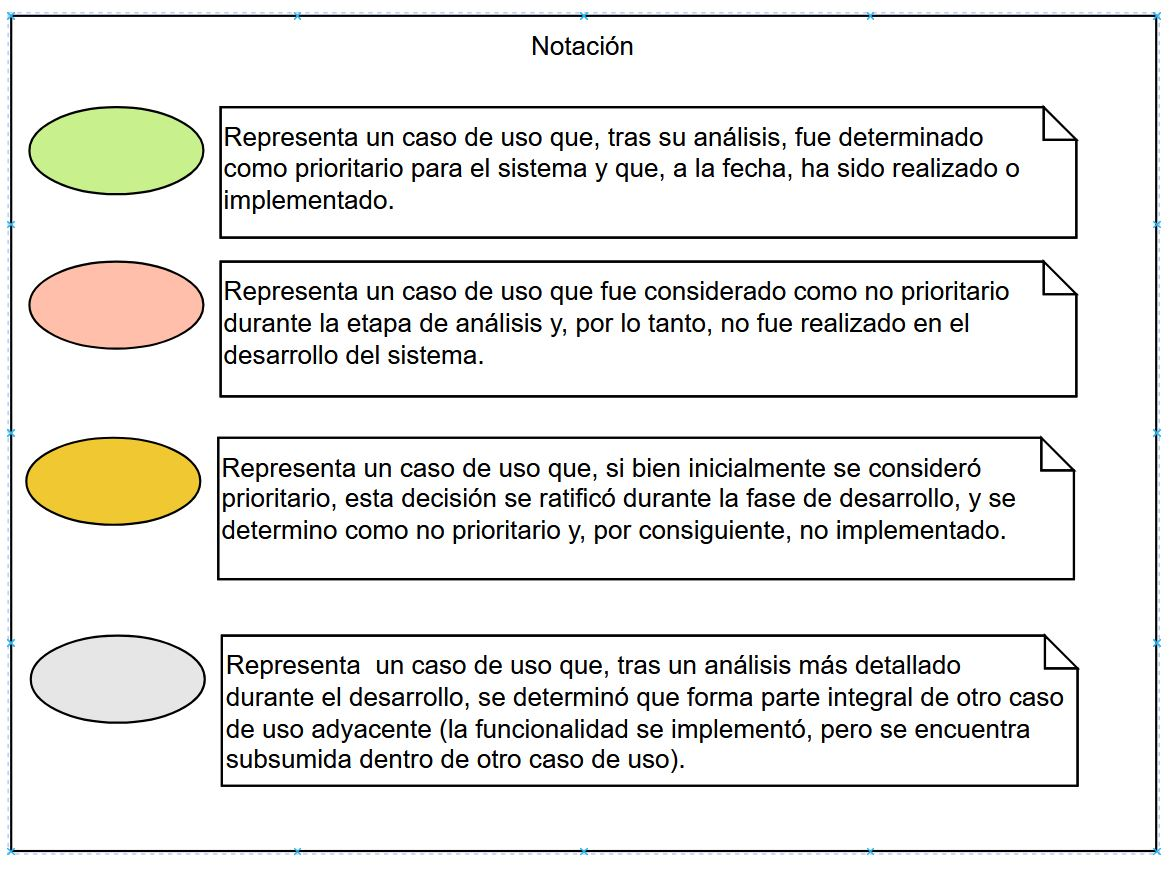
\includegraphics[width=.55\textwidth]{images/Notacion}}
		\caption{Análisis de viabilidad de los casos de uso.}
		\label{fig:Notacion}
	\end{center}
\end{figure}

A continuación, se detalla la notación empleada para la representación de los diagramas de casos de uso, la cual es fundamental para comprender la prioridad y el estado de implementación de cada funcionalidad del sistema. En la Figura \ref{fig:Notacion} se presenta la leyenda completa de esta notación, donde se utilizan cuatro colores distintos para clasificar los casos de uso según su análisis y desarrollo.


Los casos de uso representados en color verde fueron aquellos que, tras un análisis exhaustivo, se determinaron como prioritarios para la consecución de los objetivos principales del sistema y que, a la fecha, han sido completamente realizados o implementados. Esta categoría engloba las funcionalidades esenciales que sustentan la propuesta de valor de nuestro trabajo terminal.


Por otro lado, los casos de uso identificados con el color rojo fueron aquellos que, durante la etapa de análisis, se consideraron como no prioritarios para el alcance inicial del proyecto. En consecuencia, estas funcionalidades no fueron desarrolladas en la implementación del sistema.


Adicionalmente, se presenta una categoría de casos de uso en color amarillo. Estos casos fueron inicialmente considerados como prioritarios durante la fase de análisis; sin embargo, debido a diversos factores surgidos durante el desarrollo, se tomó la decisión de reconsiderar su prioridad y finalmente catalogarlos como no prioritarios, quedando fuera del alcance de la implementación actual.


Finalmente, los casos de uso representados en color gris son aquellos que, tras un análisis más detallado durante la etapa de desarrollo, se identificaron como componentes integrales de otros casos de uso adyacentes.


\subsection{Estructura de usuarios }

\begin{figure}[htbp!]
	\begin{center}
		\fbox{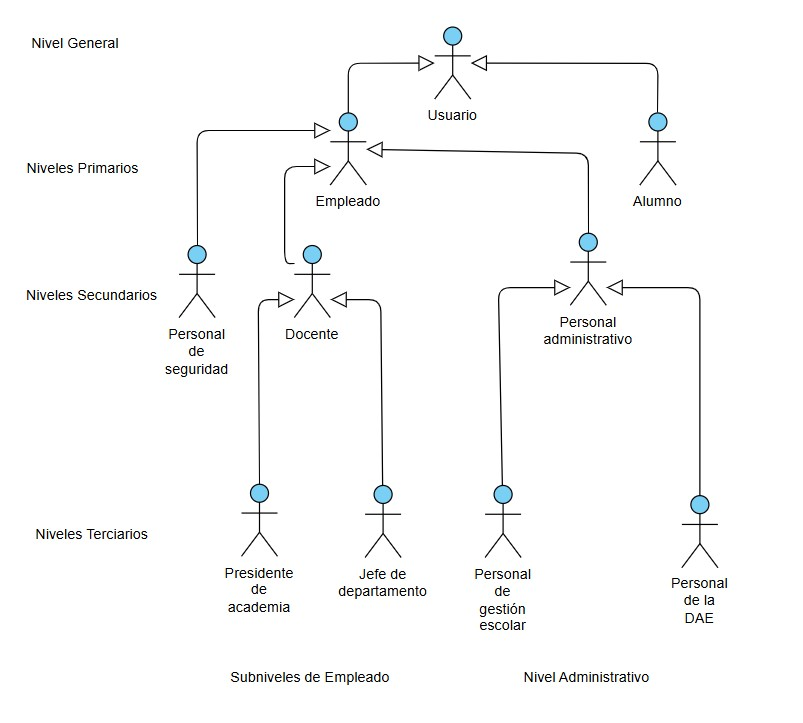
\includegraphics[width=.8\textwidth]{images/EstructuraU}}
		\caption{Estructura de los usuarios.}
		\label{fig:EstructuraU}
	\end{center}
\end{figure} 

En la Figura \ref{fig:EstructuraU} se ilustra la estructura jerárquica de los usuarios que interactúan con el sistema propuesto, detallando los diferentes tipos de roles y sus niveles de acceso. En el Nivel General, se encuentra el actor Usuario, que representa la abstracción más alta de cualquier entidad que interactúa con el sistema.

Del Usuario se derivan los Niveles Primarios: Empleado y Alumno. El Empleado engloba a todo el personal que labora en la institución, mientras que el Alumno representa a la población estudiantil.

Dentro del Nivel Primario de Empleado, encontramos los Subniveles de Empleado: Personal de seguridad y Docente. Estos roles poseen responsabilidades y permisos específicos dentro del sistema, diferenciándose de otros tipos de empleados.

También derivado del Empleado, se encuentra el Nivel Administrativo, representado por el actor Personal administrativo. Este nivel agrupa a roles con funciones de gestión y administración dentro del sistema, y se especializa en: Personal de gestión escolar, Presidente de academia, Jefe de departamento y Personal de la DAE (Dirección de administración Escolar). Cada uno de estos roles dentro del Nivel Administrativo tendrá permisos y accesos adaptados a sus responsabilidades específicas.

A continuación, se procederá a describir en detalle las responsabilidades y los procesos específicos de cada uno de los actores presentes en esta jerarquía.

%\newpage



%\newpage

%\newpage

\newpage

%---------------------------------------------------------
\subsection{Descripción de actores}

%---------------------------------------------------------
\begin{Usuario}{\hypertarget{tAlumno}{\subsubsection{Alumno}}}{
    Se refiere a las personas inscritas dentro de algún plan de estudios ofertado en la unidad académica.
}

\item[Responsabilidades:] \cdtEmpty
\begin{itemize}
    \item Asistir puntualmente a las clases, prácticas y evaluaciones.
    \item Respetar a docentes, compañeros y personal administrativo.
    \item Cumplir con los requisitos y actividades de las asignaturas inscritas, incluyendo tareas, proyectos y exámenes.
    \item Realizar oportunamente los trámites escolares como inscripciones, reinscripciones, solicitudes de documentos oficiales, etc.
    \item Portar credencial institucional en todo momento.
\end{itemize}
\textbf{Procesos clave:} \cdtEmpty
\begin{itemize}
    \item Inscribirse a asignaturas.
    \item Consultar calificaciones.
    \item Realizar pagos.
\end{itemize}
\end{Usuario}

\begin{Usuario}{\hypertarget{tPersonalSeguridad}{\subsubsection{Personal de seguridad}}}{
    Se refiere a las personas registradas como empleados y que permiten o no el acceso a la unidad académica.
}


\item[Responsabilidades:] \cdtEmpty
\begin{itemize}
    \item Supervisar el acceso y la salida de alumnos, personal docente y visitantes, asegurándose de que cumplan con los protocolos establecidos.
    \item Verificar la identificación de las personas que ingresan a las instalaciones.
    \item Responder de manera oportuna a incidentes o emergencias dentro de las instalaciones.
    \item Brindar apoyo al personal, docentes o alumnos en caso de accidentes o situaciones de riesgo.
\end{itemize}
\end{Usuario}

\begin{Usuario}{\hypertarget{tDocenteAplicador}{\subsubsection{Docente}}}{
    Se refiere a las personas registradas como empleados que dan clases a los alumnos y supervisan los ETS asignados.
}


\item[Responsabilidades:] \cdtEmpty
\begin{itemize}
    \item Impartir las clases de manera clara, puntual y completa, cumpliendo con los objetivos de aprendizaje.
    \item Diseñar y aplicar instrumentos de evaluación justos, objetivos y alineados con los contenidos del curso.
    \item Orientar a los alumnos en el desarrollo de competencias y habilidades.
    \item Resolver dudas o problemáticas académicas dentro y fuera del aula, cuando sea necesario.
    \item Registrar la asistencia de los alumnos y reportar incidencias graves.
    \item Cumplir con la entrega de calificaciones y reportes en tiempo y forma.
\end{itemize}
\end{Usuario}

\begin{Usuario}{\hypertarget{tPersonalGestion}{\subsubsection{Personal de gestión escolar}}}{
    Se refiere a las personas registradas como empleados y personal administrativo que realiza los procesos administrativos dentro de la ESCOM.
}
\item[Responsabilidades:] \cdtEmpty
\begin{itemize}
    \item Gestionar el proceso de inscripción y reinscripción de los alumnos, verificando que cumplan con los requisitos establecidos.
    \item Mantener y actualizar el historial académico de los alumnos en los sistemas institucionales.
    \item Revisar y validar actas de nacimiento, certificados y otros documentos oficiales requeridos para el registro de los alumnos.
    \item Atender solicitudes y problemáticas relacionadas con registros, certificados, bajas temporales y procesos extraordinarios.
    \item Brindar orientación a alumnos y docentes sobre trámites escolares, fechas importantes y normatividad académica.
\end{itemize}
\end{Usuario}

\begin{Usuario}{\hypertarget{tPersonalDAE}{\subsubsection{Personal de la DAE}}}{
    Se refiere a las personas registradas como empleados y personal administrativo que realiza los procesos administrativos dentro de la DAE.
}

\item[Responsabilidades:] \cdtEmpty
\begin{itemize}
    \item Fomentar y coordinar actividades extracurriculares que complementen la formación académica, como talleres, conferencias, eventos culturales y deportivos.
    \item Supervisar programas de apoyo académico, como tutorías, orientación educativa y psicológica.
    \item Difundir información sobre programas de movilidad académica, intercambios, convenios nacionales e internacionales y programas de servicio social.
    \item Gestionar y emitir las credenciales oficiales del IPN para los alumnos.
    \item Verificar que los documentos requeridos para la emisión de la credencial estén completos y sean válidos.
    \item Coordinar el proceso de inscripción de los alumnos.
    \item Actualizar y mantener los registros académicos y administrativos de los alumnos. 

\end{itemize}
\end{Usuario}


\begin{Usuario}{\hypertarget{tPresidente}{\subsubsection{Presidente de academia}}}{
Se refiere a las personas registradas como empleados y personal administrativo que lidera la academia de una unidad académica o área de conocimiento dentro de la ESCOM.
}
\item[Responsabilidades:] \cdtEmpty
\begin{itemize}
    \item Convocar y presidir las reuniones de academia, donde se toman decisiones sobre planes y programas de estudio.
    \item Coordinar la creación o actualización de planes y programas de estudio conforme a las necesidades del mercado laboral y las directrices institucionales.
    \item Verificar que los contenidos impartidos por los docentes sean consistentes con los objetivos de los programas.
    \item Detectar necesidades de capacitación entre los docentes y promover cursos o talleres. 
\end{itemize}
\end{Usuario}

\begin{Usuario}{\hypertarget{tJefe}{\subsubsection{Jefe de departamento}}}{
Se refiere a las personas registradas como empleados y personal administrativo que supervisa las actividades de una o más unidades académicas dentro de ESCOM.
}
\item[Responsabilidades:] \cdtEmpty
\begin{itemize}
\item Administrar los recursos humanos y materiales asignados al departamento.
\item Supervisar la implementación de los programas de estudio y el cumplimiento de los objetivos educativos.
\item Promover y coordinar proyectos de investigación, desarrollo tecnológico o vinculación relacionados con el departamento.
\item Atender quejas, sugerencias o problemas que surjan en el departamento, ya sea entre docentes o alumnos.
\end{itemize}
\end{Usuario}



\newpage

\subsection{Diagramas de casos de uso}

A continuación se muestran los diagramas de casos de uso:


\begin{figure}[htbp!]
	\begin{center}
		\fbox{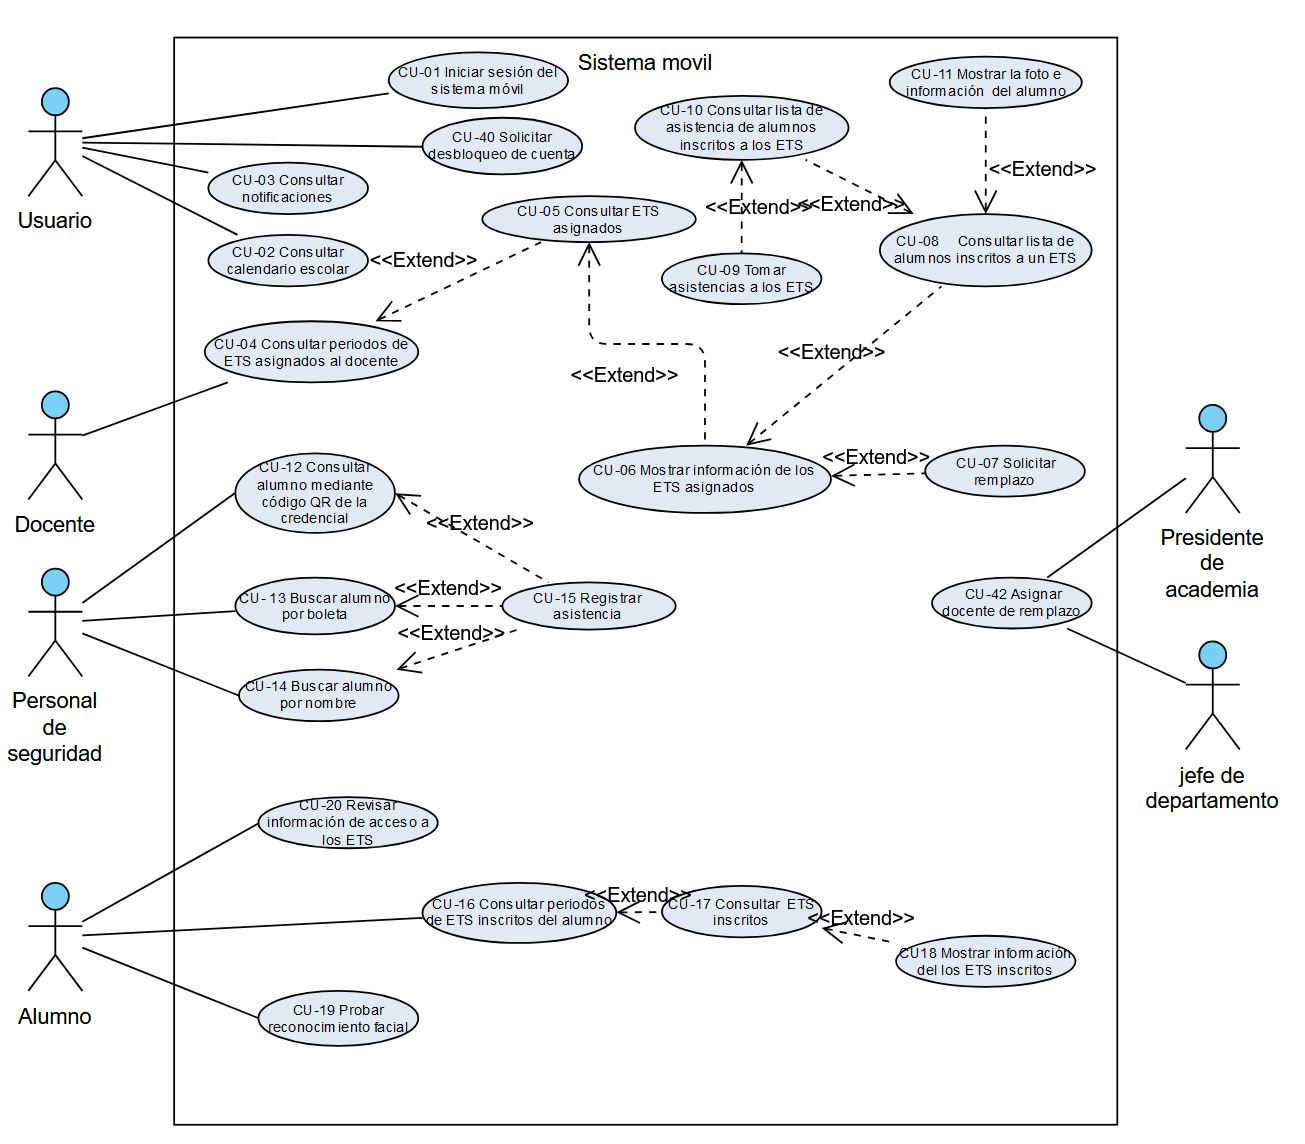
\includegraphics[width=.9\textwidth]{images/casosDeUso1}}
		\caption{Diagrama de casos de uso del sistema movil.}
		\label{fig:casosDeUso1}
	\end{center}
\end{figure}

En la Figura \ref{fig:casosDeUso1} se presenta el diagrama de casos de uso del sistema móvil, el cual constituye el núcleo central del presente trabajo terminal. Este diagrama detalla la estructura funcional del sistema, así como las interacciones específicas de los siguientes actores: Alumno, Docente, Personal de seguridad, Presidente de academia y Jefe de departamento. La notación de colores empleada en este diagrama (detallada en la Figura \ref{fig:Notacion}) permite identificar la prioridad y el estado de cada caso de uso.
Como se observa, la mayoría de los casos de uso se presentan en color verde, indicando su prioridad y realización dentro del proyecto. Sin embargo, existen algunas excepciones que merecen una explicación detallada:


El caso de uso CU-03 (Consultar notificaciones) se presenta en color amarillo. Esta decisión se tomó durante la fase de desarrollo, al identificar que su implementación completa a lo largo del ciclo de vida del proyecto presentaba una complejidad significativa. Adicionalmente, se consideró que el valor añadido de esta funcionalidad a la experiencia general del usuario no justificaba el esfuerzo requerido para su desarrollo en el alcance actual del proyecto.


Los casos de uso CU-04 (Consultar periodos de ETS asignados al docente) y CU-16 (Consultar periodos de ETS inscritos del alumno) también se identifican con el color amarillo. La determinación de no priorizar la separación de la consulta de ETS por periodos se basó en la evaluación de su impacto en la funcionalidad principal del sistema. Se concluyó que esta distinción no aportaba un valor significativo a la experiencia del usuario y que la revisión especifica de ETS por periodo carecía de relevancia práctica dentro del contexto del sistema propuesto.


El caso de uso CU-40 (Solicitar desbloqueo de cuenta) se presenta en color amarillo debido a una limitación técnica inherente a la arquitectura supuesta del sistema. Al considerar que el sistema móvil opera en conexión directa con los registros de la plataforma original del SAES (Sistema de Administración Escolar), la funcionalidad de bloquear o cambiar contraseñas desde la aplicación móvil se consideró inviable y fuera del alcance, ya que estas operaciones se gestionarían directamente a través de la plataforma original SAES.


Finalmente, el caso de uso CU-10 (Consultar lista de asistencia de alumnos inscritos al ETS) se presenta en color gris y se encuentra enlazado mediante una relación de inclusión al caso de uso CU-08 (Consultar lista de alumnos inscritos a un ETS). Esta decisión de diseño se tomó con el objetivo de optimizar la experiencia del usuario, integrando la visualización de ambas listas, es decir se muestra la lista de los alumnos inscritos al ETS y el estado de asistencia (si se presentó o no al ETS).


Los demás casos de uso presentados en color verde representan las funcionalidades prioritarias y ya implementadas del sistema móvil, las cuales serán explicadas en la sección de detalles de los casos de uso.


\newpage

%\newpage
\begin{figure}[htbp!]
	\begin{center}
		\fbox{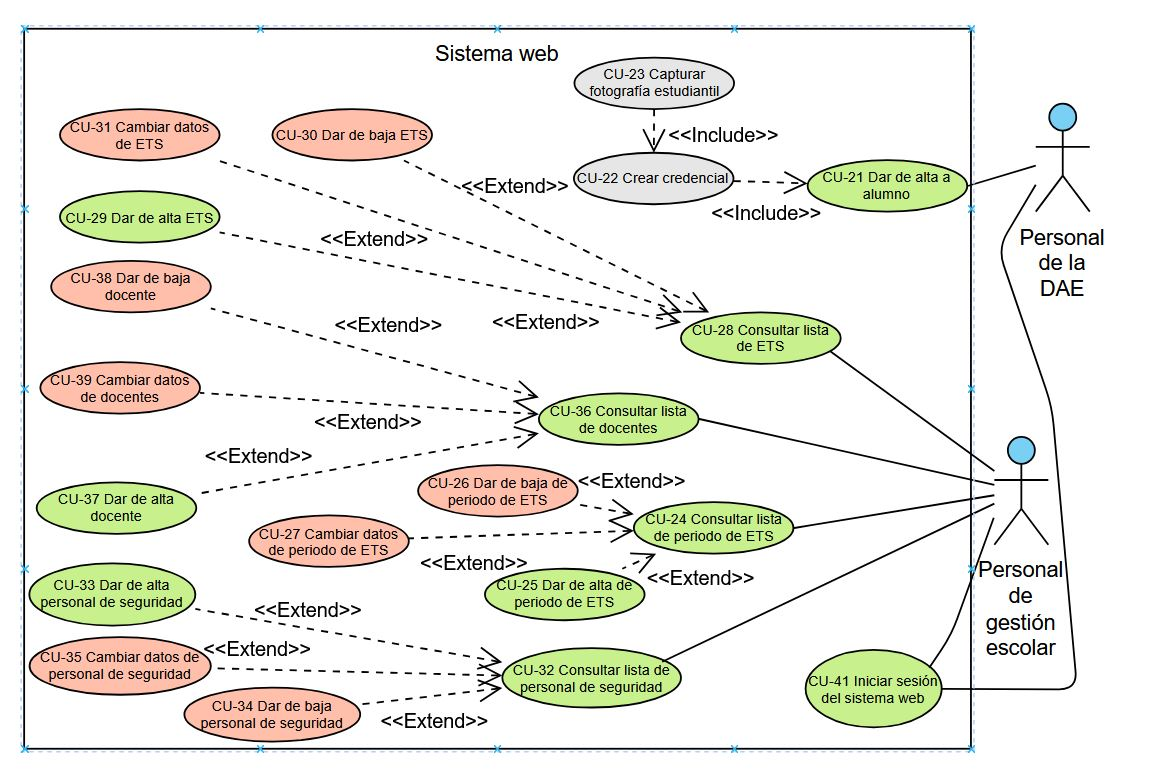
\includegraphics[width=.9\textwidth]{images/casosDeUso2}}
		\caption{Diagrama de casos de uso del sistema web.}
		\label{fig:casosDeUso2}
	\end{center}
\end{figure}


En la Figura \ref{fig:casosDeUso2} se presenta el diagrama de casos de uso correspondiente al sistema web. Este diagrama ilustra las funcionalidades a las que tienen acceso principalmente el Personal de la DAE y el Personal de gestión escolar, complementando las funcionalidades ofrecidas por el sistema móvil. Al igual que en el diagrama del sistema móvil, se utiliza la notación de colores previamente definida para indicar la prioridad y el estado de implementación de cada caso de uso.

La mayoría de los casos de uso en este diagrama se presentan en color verde, lo que indica que fueron considerados prioritarios y han sido realizados. Estos casos de uso abarcan la gestión de información y procesos administrativos relevantes para los roles del Personal de la DAE y el Personal de gestión escolar.

Sin embargo, es importante destacar la relación existente entre los casos de uso CU-21 (Dar de alta a alumno), CU-22 (Crear credencial) y CU-23 (Capturar fotografía estudiantil). Inicialmente concebidos como funcionalidades separadas, durante la fase de desarrollo se tomó la decisión de unificarlos dentro del caso de uso CU-21. Esta integración se realizó con el objetivo de optimizar la experiencia del usuario, permitiendo que el Personal de la DAE realice el alta del alumno, la captura de su fotografía y la creación de la credencial en una única pantalla o flujo de proceso. 

\subsection{Detalle de los casos de uso}

%---------------------------------------------------------
% CASOS DE USO

% !TeX root = ../ejemplo.tex

%--------------------------------------
\label{CU-01}
\begin{UseCase}{CU-01}{Iniciar sesión del sistema móvil}{
		
		Permitir que solo los usuarios registrados en el sistema móvil puedan acceder a este, además de separar completamente las funciones de los usuarios del sistema móvil.
	}
	\UCitem{Versión}{\color{Gray}1}
	\UCitem{Autor}{\color{Gray}Huertas Ramírez Daniel Martín.}
	\UCitem{Supervisa}{\color{Gray}De la Cruz de la Cruz Alejandra.}
	\UCitem{Actor}{ \hyperlink{tDocente}{Docente}, \hyperlink{tPersonalSeguridad}{Personal de seguridad}, \hyperlink{tAlumno}{Alumno}, \hyperlink{tPresidente}{Presidente de academia} y \hyperlink{tJefe}{Jefe de departamento} }
	\UCitem{Propósito}{Que el usuario del sistema móvil pueda acceder al sistema móvil y sus funciones específicas.}
	\UCitem{Entradas}{ En caso del \hyperlink{tPersonalSeguridad}{Personal de seguridad}, ingresará con su CURP y Contraseña. En caso del alumno con su Boleta y Contraseña. En caso del \hyperlink{tDocente}{Docente}, \hyperlink{tPresidente}{Presidente de academia} y \hyperlink{tJefe}{Jefe de departamento} se usará su RFC y su Contraseña}
	\UCitem{Origen}{Pantalla táctil}
	\UCitem{Salidas}{Saludo del sistema y mención de su nombre.}
	\UCitem{Destino}{Pantalla \IUref{IUE01}{Pantalla de saludo del docente} si es un docente, a la \IUref{IUE02}{Pantalla de saludo del personal de seguridad} si es un personal de seguridad, a la \IUref{IUE03}{Pantalla de saludo del alumno} si es un alumno y a la \IUref{IUE06}{Pantalla de saludo del presidente de academia/jefe de departamento} si es un presidente de academia o jefe de departamento.}
	\UCitem{Precondiciones}{El usuario debe estar registrado en el sistema móvil.}
	\UCitem{Postcondiciones}{El usuario accede al sistema móvil y podrá realizar las acciones pertinentes a su rol.}
	\UCitem{Errores}{
		E1: Cuando falte algún dato requerido entonces el sistema muestra el mensaje \textbf{``Por favor, completa todos los campos.''}
		
		E2: Cuando los datos no concuerdan con ninguna cuenta de usuario, se muestra el mensaje \textbf{ ``Datos incorrectos.''}
		
		E3: Cuando se pierde la conexión durante el proceso, los procesos se cancelan y se muestra el mensaje \textbf{ ``Conexión perdida.''}
	}
	\UCitem{Tipo}{Caso de uso primario}
	\UCitem{Observaciones}{}
\end{UseCase}
%--------------------------------------

\begin{UCtrayectoria}
	\UCpaso[\UCactor] El usuario inicia la aplicación y accede a la pantalla \IUref{IU01}{Iniciar sesión del sistema móvil}.
	\UCpaso[\UCactor] Si el usuario es un alumno, introduce su número de boleta y su contraseña. Si el usuario es Personal de seguridad, introduce su CURP y contraseña. Si el usuario es Docente, Presidente de academia o Jefe de departamento, introduce su RFC y contraseña en el sistema a través de la \IUref{IU01}{Iniciar sesión del sistema móvil}\label{CU01.introduceDatos}.
	\UCpaso[\UCactor] El usuario confirma la operación presionando el botón \IUbutton{Entrar}.
	\UCpaso El sistema verifica que todos los datos requeridos hayan sido capturados.
	\UCpaso El sistema verifica que el usuario esté registrado en el sistema.
	\UCpaso El sistema verifica que la contraseña proporcionada corresponde al usuario identificado.
	\UCpaso El sistema determina el rol del usuario que ha iniciado sesión.
	\UCpaso La sesión se inicia con éxito.
	\UCpaso El usuario es redirigido a la {Pantalla \IUref{IUE01}{Pantalla de saludo del docente} si es un docente, a la \IUref{IUE02}{Pantalla de saludo del personal de seguridad} si es un personal de seguridad, a la \IUref{IUE03}{Pantalla de saludo del alumno} si es un alumno y a la \IUref{IUE06}{Pantalla de saludo del presidente de academia/jefe de departamento} si es un presidente de academia o jefe de departamento}.
\end{UCtrayectoria}





\newpage

% !TeX root = ../ejemplo.tex

%--------------------------------------
\begin{UseCase}{CU-02}{Consultar calendario escolar}{
    Permitir que los usuarios vean el calendario escolar y puedan solicitar al sistema que les mencioné cuantos días faltan para que inicie el próximo periodo de ETS.
}
    \UCitem{Versión}{\color{Gray}1}
    \UCitem{Autor}{\color{Gray}Huertas Ramírez Daniel Martín}
    \UCitem{Supervisa}{\color{Gray}De la Cruz de la Cruz Alejandra.}
    \UCitem{Actor}{\hyperlink{Usuario}{Usuario}}
    \UCitem{Propósito}{Que el usuario consulte cuantos días faltan para el próximo periodo de ETS.}
    \UCitem{Entradas}{Ninguna}
    \UCitem{Origen}{Pantalla táctil}
    \UCitem{Salidas}{Menciona cuantos días faltan para el periodo de ETS o si menciona que ya es periodo de ETS.}
    \UCitem{Destino}{Ninguno}
    \UCitem{Precondiciones}{El usuario debe de haber iniciado sesión.}
    \UCitem{Postcondiciones}{El usuario recibe información sobre la fecha del periodo de ETS actual.}
    \UCitem{Errores}{
        E1: Cuando es periodo de ETS el sistema muestra el mensaje {\bf MSG-6}{``Actualmente es periodo de ETS.''}

        E2: Cuando no se ha establecido un periodo de ETS actual, el sistema muestra el mensaje {\bf MSG-7}{``Actualmente el periodo de ETS no ha sido establecido.''}
    
    }
    \UCitem{Tipo}{Caso de uso primario}
    \UCitem{Observaciones}{Ninguna}
\end{UseCase}
%-------------------------------------- 

\begin{UCtrayectoria}
    \UCpaso[\UCactor] El usuario accede a la pantalla \IUref{IU02}{Pantalla Consultar calendario escolar}\label{CU02.introduceDatos} para la app móvil mediante el botón con forma de calendario en cualquier pantalla excepto el inicio de sesión.
    \UCpaso[\UCactor] El usuario decide consultar cuantos días faltan para que el periodo de ETS inicie oprimiendo el botón\IUbutton{Calcular cuantos días faltan para el periodo de ETS}.
    \UCpaso El sistema calcula cuantos días faltan tomando el día actual y el día de inicio del periodo de ETS.
    \UCpaso El sistema regresa cuantos días faltan para que el periodo de ETS inicie.
    \UCpaso [\UCactor] El usuario verifica cuantos días faltan para que inicie el periodo de ETS.
\end{UCtrayectoria}








\newpage

%% !TeX root = ../ejemplo.tex

%--------------------------------------
\begin{UseCase}{CU-03}{Consultar notificaciones}{
    Permitir a los usuarios revisar sus notificaciones con más detenimiento y establecerlas como leídas.
}
    \UCitem{Versión}{\color{Gray}1}
    \UCitem{Autor}{\color{Gray}Huertas Ramírez Daniel Martín}
    \UCitem{Supervisa}{\color{Gray}De la Cruz de la Cruz Alejandra.}
    \UCitem{Actor}{\hyperlink{Usuario}{Usuario}}
    \UCitem{Propósito}{Que el usuario revise sus notificaciones con detenimiento y las establezca como leídas.}
    \UCitem{Entradas}{Ninguna}
    \UCitem{Origen}{Pantalla táctil}
    \UCitem{Salidas}{Menciona que la notificación seleccionada ha sido establecida como leída.}
    \UCitem{Destino}{Ninguno}
    \UCitem{Precondiciones}{El usuario debe de haber iniciado sesión.}
    \UCitem{Postcondiciones}{El usuario revisó sus notificaciones.}
    \UCitem{Errores}{
        E1: Cuando el usuario no tiene notificaciones el sistema muestra el mensaje {\bf MSG-8}{``Actualmente no hay notificaciones.''}    
    }
    \UCitem{Tipo}{Caso de uso primario}
    \UCitem{Observaciones}{}

\end{UseCase}
%-------------------------------------- 

\begin{UCtrayectoria}
    \UCpaso[\UCactor] El usuario accede a la pantalla \IUref{IU03}{Pantalla Consultar notificaciones}\label{CU03.introduceDatos} para la app móvil  mediante el botón con forma de campana en cualquier pantalla excepto los inicios de sesión.
    \UCpaso[\UCactor] El usuario decide consultar sus notificaciones más actuales \Trayref{A}.
    \UCpaso[\UCactor] El usuario marco como leídas las notificaciones que acaba de leer mediante el botón con forma de palomita especifico de cada notificación.
    \UCpaso El sistema marca como leídas las notificaciones.

\end{UCtrayectoria}

\begin{UCtrayectoriaA}{A}{El usuario quiere consultar las notificaciones de una fecha específica}
	\UCpaso[\UCactor] El usuario usa el buscador de la parte superior para buscar notificaciones según su fecha.
	\UCpaso[\UCactor] El usuario marco como leídas las notificaciones que acaba de leer mediante el botón con forma de palomita especifico de cada notificación.
	\UCpaso El sistema marca como leídas las notificaciones.

\end{UCtrayectoriaA}



%\newpage

%% \IUref{IUAdmPS}{Administrar Planta de Selección}
% \IUref{IUModPS}{Modificar Planta de Selección}
% \IUref{IUEliPS}{Eliminar Planta de Selección}

%-------------------------------------- COMIENZA descripción del caso de uso.

%\begin{UseCase}[archivo de imágen]{UCX}{Nombre del Caso de uso}{
%--------------------------------------
% !TeX root = ../ejemplo.tex
\begin{UseCase}{CU-04}{Consultar periodos de ETS asignados al docente}{
	Este caso de uso permite al docente consultar los periodos de ETS que tiene asignados. 
}
\UCitem{Versión}{\color{Gray}1.0} 
\UCitem{Autor}{\color{Gray}De la cruz De la cruz Alejandra}
\UCitem{Supervisa}{\color{Gray}Huertas Ramírez Daniel Martín }
\UCitem{Actor}{\hyperlink{Docente}{Docente}}
\UCitem{Propósito}{Permitir al docente consultar los periodos de ETS que le han sido asignados.}
\UCitem{Entradas}{Ninguna}
\UCitem{Origen}{Pantalla táctil}
\UCitem{Salidas}{Lista de periodos de ETS asignados.}
\UCitem{Destino}{\IUref{IU04}{Pantalla Periodo de ETS}}
\UCitem{Precondiciones}{El docente debe estar autenticado en el sistema.}
\UCitem{Postcondiciones}{El docente ha consultado los periodos de ETS asignados.}
\UCitem{Errores}{
		E1: El sistema no puede recuperar la información de los periodos y muestra el mensaje {\bf MSG-9}{``Error al consultar la base de datos. Intente nuevamente más tarde''.}
		
		E2: No hay periodos de ETS asignados al docente y se muestra el mensaje {\bf MSG-10}{``No tienes periodos de ETS asignados.''}
}
\UCitem{Tipo}{Se entiende del CU-01 Iniciar sesión del sistema móvil}
\UCitem{Observaciones}{Ninguna}
\end{UseCase}
%--------------------------------------
\begin{UCtrayectoria}
\UCpaso[\UCactor] El docente accede a la \IUref{IUE01}{Pantalla saludo del docente} después de haber iniciado sesión.
\UCpaso[\UCactor] El docente presiona el botón \IUbutton{Consultar periodos de ETS}.
\UCpaso El sistema verifica que el docente cuente con periodos de ETS. \Trayref{A}.
\UCpaso El sistema busca en la base de datos los periodos de ETS asignados al docente.
\UCpaso El sistema despliega la lista de periodos de ETS asignados al docente en la \IUref{IU04}{Pantalla Periodo de ETS}.
\end{UCtrayectoria}
%--------------------------------------        
\begin{UCtrayectoriaA}{A}{No hay periodos asignados al docente}
\UCpaso El sistema verifica y no encuentra registros de periodos de ETS asignados al docente.
\UCpaso El sistema muestra un mensaje: {\bf MSG-10}{`` No tienes periodos de ETS asignados.''}
\UCpaso[\UCactor] El docente presiona el botón \IUbutton{Regresar} para volver a la pantalla anterior.
\UCpaso Fin de la trayectoria alternativa.
\end{UCtrayectoriaA}
%--------------------------------------        
\begin{UCtrayectoriaA}{B}{Error en la conexión con la base de datos}
\UCpaso El sistema muestra un mensaje de error: {\bf MSG-9}{``Error al consultar la base de datos. Intente nuevamente más tarde.''}
\UCpaso[\UCactor] El docente resiona el botón \IUbutton{Aceptar} para cerrar el mensaje.
\UCpaso[\UCactor] El docente puede intentar la consulta nuevamente o presionar el botón \IUbutton{Regresar} para volver a la pantalla anterior.
\UCpaso Fin de la trayectoria alternativa.
\end{UCtrayectoriaA}
%-------------------------------------- TERMINA descripción del caso de uso.

%\newpage

% \IUref{IUAdmPS}{Administrar Planta de Selección}
% \IUref{IUModPS}{Modificar Planta de Selección}
% \IUref{IUEliPS}{Eliminar Planta de Selección}

%-------------------------------------- COMIENZA descripción del caso de uso.

%\begin{UseCase}[archivo de imágen]{UCX}{Nombre del Caso de uso}{
%--------------------------------------
\label{CU-05}
\begin{UseCase}{CU-05}{Consultar ETS asignados}{
		Este caso de uso permite al docente consultar los ETS que tiene asignados.
	}
	\UCitem{Versión}{\color{Gray}2.0}
	\UCitem{Autor}{\color{Gray}De la cruz De la cruz Alejandra}
	\UCitem{Supervisa}{\color{Gray}Huertas Ramírez Daniel Martín}
	\UCitem{Actor}{\hyperlink{tDocente}{Docente}}
	\UCitem{Propósito}{Permitir al docente consultar los ETS que le han sido asignados.}
	\UCitem{Entradas}{Solicitud de consulta.}
	\UCitem{Origen}{Pantalla táctil}
	\UCitem{Salidas}{Lista de ETS asignados (Unidad de Aprendizaje, Periodo, Fecha, Turno) o indicación de que no hay ETS asignados.}
	\UCitem{Destino}{\IUref{IU06}{Pantalla de Consultar ETS}}
	\UCitem{Precondiciones}{El docente debe haber iniciado sesión en el sistema (\textbf{\hyperref[CU-01]{CU-01 Iniciar sesión del sistema móvil}}).}
	\UCitem{Postcondiciones}{El docente ha consultado los ETS asignados.}
	\UCitem{Errores}{
		E1: El sistema no puede recuperar la información de los ETS asignados y se muestra el mensaje \textbf{``Error al consultar la base de datos. Intente nuevamente más tarde.''}.
		
		E2: Cuando se pierde la conexión durante el proceso, los procesos se cancelan y se muestra el mensaje \textbf{ ``Conexión perdida.''}
	}
	\UCitem{Tipo}{Caso de uso primario}
	\UCitem{Observaciones}{Ninguna}
\end{UseCase}
%--------------------------------------
\begin{UCtrayectoria}
	\UCpaso[\UCactor] El docente accede a la \IUref{IU05}{Pantalla de Consultar ETS} desde el menú principal.
	\UCpaso El sistema recupera la lista de todos los ETS asignados al docente.
	\UCpaso El sistema muestra la lista de ETS, incluyendo para cada uno: Unidad de Aprendizaje, Periodo, Fecha y Turno.
	\UCpaso[\UCactor] El docente visualiza la lista de ETS asignados.
	\UCpaso[\UCactor] El docente selecciona un ETS de la lista.
	\UCpaso El sistema redirige al docente a la pantalla \IUref{IU06}{Pantalla Información de ETS}.
	\UCpaso[\UCactor] Opcionalmente, el docente puede presionar el botón \IUbutton{Todos} para ver todos los ETS asignados.
	\UCpaso[\UCactor] Opcionalmente, el docente puede presionar el botón \IUbutton{Mis ETS} para ver los ETS que tiene pendientes por aplicar o supervisar.
\end{UCtrayectoria}

%--------------------------------------
\begin{UCtrayectoriaA}{A}{No hay ETS asignados}
	\UCpaso El sistema verifica que no hay ETS asignados al docente.
	\UCpaso El sistema muestra el mensaje \textbf{``No hay ETS creados.''} indicando que no hay ETS asignados.
	\UCpaso[\UCactor] El docente visualiza el mensaje.
	\UCpaso[\UCactor] El docente presiona el botón \IUbutton{Regresar} para volver a la pantalla anterior.
	\UCpaso Fin de la trayectoria alternativa.
\end{UCtrayectoriaA}

%--------------------------------------
\begin{UCtrayectoriaA}{B}{Error en la conexión con la base de datos}
	\UCpaso El sistema intenta recuperar la lista de ETS asignados.
	\UCpaso Ocurre un error en la conexión con la base de datos.
	\UCpaso El sistema muestra el mensaje de error: \textbf{``Error al consultar la base de datos. Intente nuevamente más tarde.''}.
	\UCpaso[\UCactor] El docente presiona el botón \IUbutton{Aceptar} para cerrar el mensaje.
	\UCpaso[\UCactor] El docente puede intentar la consulta nuevamente o presionar el botón \IUbutton{Regresar} para volver a la pantalla anterior.
	\UCpaso Fin de la trayectoria alternativa.
\end{UCtrayectoriaA}

%-------------------------------------- TERMINA descripción del caso de uso.
\newpage

% \IUref{IUAdmPS}{Administrar Planta de Selección}
% \IUref{IUModPS}{Modificar Planta de Selección}
% \IUref{IUEliPS}{Eliminar Planta de Selección}

%-------------------------------------- COMIENZA descripción del caso de uso.

%\begin{UseCase}[archivo de imágen]{UCX}{Nombre del Caso de uso}{
%--------------------------------------
% !TeX root = ../ejemplo.tex
\begin{UseCase}{CU-06}{Mostrar información de los ETS asignados}{
	Este caso de uso permite al docente visualizar la información detallada de los ETS que tiene asignados.
}
\UCitem{Versión}{\color{Gray}1.0}
\UCitem{Autor}{\color{Gray}De la cruz De la cruz Alejandra}
\UCitem{Supervisa}{\color{Gray}Huertas Ramírez Daniel Martín}
\UCitem{Actor}{\hyperlink{PersonalAcademico}{Docente}}
\UCitem{Propósito}{Permite al docente visualizar la información detallada de cada ETS que tiene asignado.}
\UCitem{Entradas}{Ninguna}
\UCitem{Origen}{Pantalla táctil}
\UCitem{Salidas}{Detalle de ETS asignado.}
\UCitem{Destino}{\IUref{IU06}{Pantalla Información de ETS}}
\UCitem{Precondiciones}{El docente debe estar autenticado y tener ETS asignados en el sistema.}
\UCitem{Postcondiciones}{El docente ha visualizado la información detallada de sus ETS asignados.}
\UCitem{Errores}{
		E1: El sistema no puede recuperar la información detallada de los ETS y muestra el mensaje {\bf MSG-12}{``Información no disponible para el ETS seleccionado''}.
		E2: Error en la conexión con la base de datos y muestra el mensaje y muestra el mensaje {\bf MSG-9}{``Error al consultar la base de datos. Intente nuevamente más tarde.''}.
}
\UCitem{Tipo}{Se entiende del CU-05 Mostrar información de los ETS asignados}
\UCitem{Observaciones}{Ninguna}
\end{UseCase}
%--------------------------------------
\begin{UCtrayectoria}
\UCpaso[\UCactor] El docente selecciona el ETS que desea visualizar desde la \IUref{IU05}{Pantalla  Consultar ETS}.
\UCpaso[\UCsist] El sistema verifica si existen detalles disponibles para el ETS seleccionado. \Trayref{A}
\UCpaso El sistema despliega la información detallada de cada ETS asignado en la \IUref{IU06}{Pantalla Información de ETS}
\end{UCtrayectoria}
%--------------------------------------        
\begin{UCtrayectoriaA}{A}{No hay detalles disponibles para el ETS seleccionado}
\UCpaso El sistema muestra un mensaje: {\bf MSG-12}{``Información no disponible para el ETS seleccinado''}
\UCpaso[\UCactor] El docente presiona el botón \IUbutton{Regresar} para volver a la lista de ETS.
\UCpaso Fin de la trayectoria alternativa.
\end{UCtrayectoriaA}

%--------------------------------------        
\begin{UCtrayectoriaA}{B}{Error en la conexión con la base de datos}
\UCpaso El sistema muestra un mensaje de error: {\bf MSG-9}{``Error al consultar la base de datos. Intente nuevamente más tarde.''}
\UCpaso[\UCactor] El docente presiona el botón \IUbutton{Aceptar} para cerrar el mensaje.
\UCpaso[\UCactor] El docente puede intentar la consulta nuevamente o presionar el botón \IUbutton{Regresar} para volver a la pantalla anterior.
\UCpaso Fin de la trayectoria alternativa.
\end{UCtrayectoriaA}

%-------------------------------------- TERMINA descripción del caso de uso.


\newpage

% \IUref{IUAdmPS}{Administrar Planta de Selección}
% \IUref{IUModPS}{Modificar Planta de Selección}
% \IUref{IUEliPS}{Eliminar Planta de Selección}

%-------------------------------------- COMIENZA descripción del caso de uso.

%\begin{UseCase}[archivo de imágen]{UCX}{Nombre del Caso de uso}{
%--------------------------------------
\begin{UseCase}{CU-07}{Solicitar remplazo }{
	Este caso de uso permite a un docente solicitar un reemplazo para que aplique el ETS cuando no pueda asistir.
}
\UCitem{Versión}{\color{Gray}1.0}
\UCitem{Autor}{\color{Gray}De la cruz De la cruz Alejandra}
\UCitem{Supervisa}{\color{Gray}Huertas Ramírez Daniel}
\UCitem{Actor}{\hyperlink{PersonalAcademico}{Docente}}
\UCitem{Propósito}{Permitir al docente responsable de un ETS solicitar apoyo de otro profesor para llevar a cabo la aplicación, notificando al jefe de departamento o al presidente de academia.}
\UCitem{Entradas}{Identificador del ETS y razón por la que se pide el remplazo.}
\UCitem{Origen}{Pantalla táctil}
\UCitem{Salidas}{
	Se muestra el mensaje \textbf{``Solicitud exitosa. La solicitud de reemplazo ha sido registrada correctamente'', indicando que la solicitud fue enviada con éxito.}
	
	Se muestra el mensaje \textbf{: ``Ya existe una solicitud pendiente para este ETS'', indicando que ya se ha realizado una solicitud previa para el ETS.}
	}
\UCitem{Destino}{\IUref{IU06}{Pantalla Información de ETS}}
\UCitem{Precondiciones}{El docente debe estar autenticado en el sistema y tener un ETS asignado.}
\UCitem{Postcondiciones}{La solicitud ha sido enviada al jefe de departamento y/o al presidente de academia.}
\UCitem{Errores}{
	E1: Cuando se pierde la conexión durante el proceso, los procesos se cancelan y se muestra el mensaje {\bf  ``Error al enviar la solicitud''}
}
\UCitem{Tipo}{Se entiende del CU-06 Mostrar información de los ETS asignados}
\UCitem{Observaciones}{Ninguna}
\end{UseCase}
%--------------------------------------
\begin{UCtrayectoria}
\UCpaso[\UCactor] El docente accede a la \IUref{IU06}{Pantalla Información de ETS}.
\UCpaso[\UCactor] El docente selecciona la opción \IUbutton{Solicitar reemplazo} para el ETS asignado.
\UCpaso El sistema redirige al docente a la pantalla \IUref{IU07}{ Solicitar remplazo }.
\UCpaso El sistema muestra el ETS selecciona.
\UCpaso[\UCactor] El docente ingresa la razón para solicitar el remplazo.
\UCpaso[\UCactor] El docente oprime el botón \IUbutton{Enviar solicitud} [Trayectoria A] [Trayectoria B] .
\UCpaso El sistema envía la solicitud de remplazo al jefe de departamento y/o al presidente de academia.
\end{UCtrayectoria}
%--------------------------------------        
\begin{UCtrayectoriaA}{A}{Ya existe una solicitud pendiente para el ETS}
	\UCpaso El sistema valida que exista una solicitud previa no resuelta.
	\UCpaso El sistema muestra el mensaje: {\bf``Ya existe una solicitud pendiente para este ETS''}.
	\UCpaso[\UCactor] El docente presiona \IUbutton{Aceptar} para regresar a \IUref{IU06}{Pantalla Información de ETS}.
\end{UCtrayectoriaA}
%-------------------------------------- TERMINA descripción del caso de uso.
\begin{UCtrayectoriaA}{B}{Error al enviar la solicitud}
	\UCpaso El sistema detecta un fallo en el servidor o conexión.
	\UCpaso Muestra el mensaje: {\bf``Error al enviar la solicitud''}.
	\UCpaso[\UCactor] El docente selecciona:
	\begin{itemize}
		\item \IUbutton{Cancelar} para volver a \IUref{IU06}{Pantalla Información de ETS}.
	\end{itemize}
\end{UCtrayectoriaA}

\newpage

% \IUref{IUAdmPS}{Administrar Planta de Selección}
% \IUref{IUModPS}{Modificar Planta de Selección}
% \IUref{IUEliPS}{Eliminar Planta de Selección}

%-------------------------------------- COMIENZA descripción del caso de uso.

%\begin{UseCase}[archivo de imágen]{UCX}{Nombre del Caso de uso}{
%--------------------------------------
\label{CU-08}
\begin{UseCase}{CU-08}{Consultar lista de alumnos inscritos a un ETS}{
		Este caso de uso permite al docente consultar la lista de los alumnos inscritos a un ETS asignado.
		
		Ademas, el caso de uso CU-10 (Consultar lista de asistencia de alumnos inscritos a los ETS) se ha unificado con CU-08 (Consultar lista de alumnos inscritos a un ETS) para mejorar la eficiencia y la experiencia del usuario. La funcionalidad de visualización de la asistencia, previamente contemplada en CU-10, se integra ahora directamente en la \IUref{IU08}{Pantalla Lista de asistencia de ETS} de CU-08, presentando la lista de alumnos y su estado de asistencia en una única interfaz.
	}
	\UCitem{Versión}{\color{Gray}2.0}
	\UCitem{Autor}{\color{Gray}De la cruz De la cruz Alejandra}
	\UCitem{Supervisa}{\color{Gray}Huertas Ramírez Daniel Martín}
	\UCitem{Actor}{\hyperlink{tDocente}{Docente}}
	\UCitem{Propósito}{Permitir al docente visualizar la lista de alumnos inscritos en un ETS para verificar su asistencia y acceder a la creación de reportes dentro del periodo permitido.}
	\UCitem{Entradas}{Solicitud de ver la lista de alumnos.}
	\UCitem{Origen}{\IUref{IU06}{Pantalla Información de ETS}}
	\UCitem{Salidas}{Lista de los alumnos inscritos al ETS (Boleta y Nombre) junto con un icono representativo del estado de su asistencia. Mensajes informativos sobre el periodo de reporte y permisos.}
	\UCitem{Destino}{\IUref{IU08}{Pantalla Lista de asistencia de ETS}.}
	\UCitem{Precondiciones}{El docente debe haber iniciado sesión (\textbf{\hyperref[cu:CU-01]{CU-01 Iniciar sesión del sistema móvil}}) y haber consultado la información detallada del ETS (\textbf{\hyperref[cu:CU-06]{CU-06 Mostrar información de los ETS asignados}}).}
	\UCitem{Postcondiciones}{El docente ha visualizado la lista de asistencia de los alumnos inscritos al ETS y puede acceder a la creación de reportes si se encuentra dentro del periodo permitido y tiene los permisos necesarios.}
	\UCitem{Errores}{
		E1: El sistema pierde la conexión al intentar recuperar la lista de asistencia y se muestra el mensaje \textbf{ ``Error al consultar la base de datos. Intente nuevamente más tarde.''}.
	}
	\UCitem{Tipo}{Caso de uso primario}
	\UCitem{Observaciones}{Cada alumno en la lista se presenta con dos botones: uno con su boleta y nombre, y otro con un icono representativo de su estado de asistencia. El botón con la boleta y nombre del alumno redirige a la \textbf{Pantalla Reporte} (\IUref{IUE07}{Creación del reporte}). El botón con el icono redirige a la \IUref{IU20}{Pantalla mostrar la foto e información del alumno} **solo si la hora actual se encuentra entre 10 minutos antes del inicio del ETS y 2 horas después del inicio del ETS.** Si se quiere conocer todos los iconos y su significado, porfavor revisar \textbf{\hyperref[sec:tablaIconosAsistencia]{Tabla de Iconos de Estado de Asistencia}.}}
\end{UseCase}
%--------------------------------------
\begin{UCtrayectoria}
	\UCpaso[\UCactor] El docente presiona el botón \IUbutton{Ir a la lista de alumnos} desde la pantalla \IUref{IU06}{Pantalla Información de ETS}.
	\UCpaso El sistema verifica la existencia del ETS. \Trayref{C}
	\UCpaso El sistema recupera la lista de alumnos inscritos en el ETS junto con su estado de asistencia. \Trayref{A}, \Trayref{B}
	\UCpaso El sistema muestra la lista de alumnos en la \IUref{IU08}{Pantalla Lista de asistencia de ETS}. Cada alumno se muestra con un botón que contiene su boleta y nombre (habilitado según el periodo de reporte y rol del docente), y un botón con el icono representativo de su estado de asistencia.
	\UCpaso[\UCactor] El docente visualiza la lista de alumnos.
	\UCpaso Para cada alumno, el sistema verifica si la hora actual se encuentra dentro del periodo permitido para generar reportes (10 minutos antes hasta 2 horas después del inicio del ETS). \Trayref{D}, \Trayref{E}
	\UCpaso El sistema verifica si el docente es el aplicador del ETS para el alumno seleccionado antes de permitir el acceso a la creación del reporte. \Trayref{F}
	\UCpaso[\UCactor] Si el periodo es válido y el docente es el aplicador, al presionar el botón con la boleta y nombre del alumno, el sistema lo redirige a la \textbf{Pantalla Reporte} (\IUref{IUE07}{Creación del reporte}).
	\UCpaso[\UCactor] Al presionar el botón con el icono, el sistema lo redirige a la \IUref{IU20}{Pantalla mostrar la foto e información del alumno}.
\end{UCtrayectoria}

%--------------------------------------
\begin{UCtrayectoriaA}{A}{El ETS no tiene alumnos inscritos}
	\UCpaso El sistema muestra el mensaje: \textbf{ ``No hay alumnos inscritos al ETS.''}.
	\UCpaso[\UCactor] El docente presiona el botón \IUbutton{Regresar} para volver a la pantalla \IUref{IU06}{Pantalla Información de ETS}.
	\UCpaso Fin de la trayectoria alternativa.
\end{UCtrayectoriaA}
%--------------------------------------
\begin{UCtrayectoriaA}{B}{Error en la conexión con la base de datos}
	\UCpaso El sistema intenta recuperar la lista de alumnos inscritos.
	\UCpaso Ocurre un error en la conexión con la base de datos.
	\UCpaso El sistema muestra el mensaje de error: \textbf{ ``Error al consultar la base de datos. Intente nuevamente más tarde.''}.
	\UCpaso[\UCactor] El docente presiona el botón \IUbutton{Aceptar} para cerrar el mensaje.
	\UCpaso[\UCactor] El docente puede intentar la consulta nuevamente.
	\UCpaso Fin de la trayectoria alternativa.
\end{UCtrayectoriaA}
%--------------------------------------
\begin{UCtrayectoriaA}{C}{El ETS no existe}
	\UCpaso El sistema no encuentra el ETS correspondiente.
	\UCpaso El sistema muestra el mensaje de error: \textbf{ ``El ETS seleccionado no es válido.''}.
	\UCpaso[\UCactor] El docente presiona el botón \IUbutton{Regresar} para volver a la pantalla \IUref{IU06}{Pantalla Información de ETS}.
	\UCpaso Fin de la trayectoria alternativa.
\end{UCtrayectoriaA}
%--------------------------------------
\begin{UCtrayectoriaA}{D}{Aún no es periodo para crear reportes}
	\UCpaso El sistema verifica que la hora actual es anterior a 10 minutos antes de la hora de inicio del ETS.
	\UCpaso El sistema muestra el mensaje: \textbf{ ``Aún no es periodo para crear los reportes. Faltan (tiempo)''}.
	\UCpaso El botón con la boleta y nombre del alumno se muestra deshabilitado o no interactivo.
	\UCpaso[\UCactor] El docente visualiza el mensaje.
	\UCpaso Fin de la trayectoria alternativa.
\end{UCtrayectoriaA}
%--------------------------------------
\begin{UCtrayectoriaA}{E}{El periodo para registrar los reportes ha concluido}
	\UCpaso El sistema verifica que la hora actual es posterior a 2 horas después de la hora de inicio del ETS.
	\UCpaso El sistema muestra el mensaje: \textbf{ ``El periodo para registrar los reportes ha concluido.''}.
	\UCpaso El botón con la boleta y nombre del alumno se muestra deshabilitado o no interactivo.
	\UCpaso[\UCactor] El docente visualiza el mensaje.
	\UCpaso Fin de la trayectoria alternativa.
\end{UCtrayectoriaA}
%--------------------------------------
\begin{UCtrayectoriaA}{F}{Docente no autorizado para ver información del alumno}
	\UCpaso El sistema verifica que el docente no es el aplicador del ETS para el alumno seleccionado.
	\UCpaso El sistema muestra el mensaje: \textbf{ ``Usted no está autorizado para crear el reporte de este alumno.''}.
	\UCpaso El botón con la boleta y nombre del alumno se muestra deshabilitado o no interactivo.
	\UCpaso[\UCactor] El docente visualiza el mensaje.
	\UCpaso Fin de la trayectoria alternativa.
\end{UCtrayectoriaA}

%-------------------------------------- TERMINA descripción del caso de uso.

\newpage

% \IUref{IUAdmPS}{Administrar Planta de Selección}
% \IUref{IUModPS}{Modificar Planta de Selección}
% \IUref{IUEliPS}{Eliminar Planta de Selección}

%-------------------------------------- COMIENZA descripción del caso de uso.

%\begin{UseCase}[archivo de imágen]{UCX}{Nombre del Caso de uso}{
%--------------------------------------
\label{CU-09}
\begin{UseCase}{CU-09}{Tomar asistencias a los ETS}{
		Este caso de uso permite al docente registrar la asistencia o una incidencia para los alumnos inscritos a un ETS asignado, utilizando diferentes métodos de verificación y detallando la razón en caso de incidencia.
	}
	\UCitem{Versión}{\color{Gray}2.0}
	\UCitem{Autor}{\color{Gray}De la cruz De la cruz Alejandra}
	\UCitem{Supervisa}{\color{Gray}Huertas Ramírez Daniel Martín}
	\UCitem{Actor}{\hyperlink{tDocente}{Docente}}
	\UCitem{Propósito}{Permitir al docente registrar la asistencia (aceptado) o una incidencia (rechazado) de los alumnos inscritos a un ETS, utilizando verificación por credencial QR, reconocimiento facial o confirmación manual, con la opción de detallar la razón de la incidencia.}
	\UCitem{Entradas}{Selección de un alumno desde la \IUref{IU08}{Lista de asistencia de ETS.}}
	\UCitem{Origen}{\IUref{IU08}{Lista de asistencia de ETS}}
	\UCitem{Salidas}{Presentación de la credencial simulada del alumno, opciones de verificación (QR y Reconocimiento Facial), botones para registrar asistencia o incidencia, mensajes de éxito o error en la verificación y registro.}
	\UCitem{Destino}{\IUref{IUE07}{Creación del reporte}}
	\UCitem{Precondiciones}{El docente debe haber iniciado sesión (\textbf{\hyperref[CU-01]{CU-01 Iniciar sesión del sistema móvil}}) y haber consultado la lista de alumnos inscritos al ETS (\textbf{\hyperref[CU-08]{CU-08 Consultar lista de alumnos inscritos a un ETS}}).}
	\UCitem{Postcondiciones}{La asistencia o incidencia del alumno ha sido registrada en el sistema para el ETS. En caso de eliminación de un reporte existente, la pantalla se recarga.}
	\UCitem{Errores}{
		
			E1: Cuando no se encuentra los datos del alumno \textbf{ ``No se encontraron datos.``}
			
			E2: Cuando el código QR no es valido se muestra el mensaje \textbf{ ``Código QR no válido.``}
			
			E3: Cuando no se pudo capturar la foto se  muestra el mensaje \textbf{ ``Error al capturar la fotografía.``}
			
			E4: Cuando no se pudo realizar el reconocimiento facial se muestra el mensaje\textbf{ ``Error al realizar el reconocimiento facial.``}
			
			E5: Cuando hay un error de conexión se muestra el mensaje \textbf{ ``Error de conexión.``}
			
			E6: Cuando ocurre un error general se muestra el mensaje \textbf{ ``Ocurrió un fallo en el proceso.``}
			
			E7: Cuando el docente no elije un tipo para crear el reporte se muestra el mensaje \textbf{ ``Debe seleccionar un tipo.``}
			
			E8: Cuando el docente intenta hacer un reporte con IA, pero no ha pasado por el reconocimiento facial se muestra el mensaje \textbf{ ``Para hacer un reporte de reconocimiento facial necesita haber hecho el proceso de verificar con IA.``}
			
			E9: Cuando falta un campo por llenar o mas en la creación del reporte se muestra el mensaje \textbf{ ``Debe completar todos los campos correctamente.``}
			
			E10: Cuando falla la creación del reporte de asistencia se muestra el mensaje \textbf{ ``Error al crear el reporte de asistencia.``}
			
			E11: Cuando falla la creación del reporte de incidencia se muestra el mensaje \textbf{ ``Error al crear el reporte de incidencia.``}
			
			E12: Cuando la razón tiene menos de 5 letras se muestra el mensaje\textbf{ ``La razón debe tener al menos 5 letras.``}
		
	}
	\UCitem{Tipo}{Caso de uso primario}
	\UCitem{Observaciones}{Si ya existe un reporte para el alumno, se pregunta al docente si desea eliminarlo. La precisión y la foto del reconocimiento facial se muestran al final de la pantalla si el proceso fue exitoso.}
\end{UseCase}
%--------------------------------------
\begin{UCtrayectoria}
	\UCpaso[\UCactor] El docente selecciona un alumno de la lista en la \IUref{IU08}{Lista de asistencia de ETS}.
	\UCpaso El sistema muestra la \IUref{IUE07}{Creación del reporte} con la simulación de la credencial del alumno. \Trayref{A}
	\UCpaso[\UCactor] El docente puede optar por:
	\begin{itemize}
		\item Verificar con Código QR: Presiona \IUbutton{Verificar con QR} \Trayref{B}.
		\item Verificar con IA (Reconocimiento Facial): Presiona \IUbutton{Verificar con IA} \Trayref{C}.
		\item Registrar asistencia o incidencia directamente (si está seguro de la identidad) \Trayref{D}, \Trayref{E}.
	\end{itemize}
	\UCpaso[\UCactor] El docente selecciona un tipo de registro (Aceptado o Rechazado) y, si es rechazado, escribe una razón. \Trayref{F}
	\UCpaso[\UCactor] El docente presiona el botón \IUbutton{Registrar asistencia} o \IUbutton{Registrar incidencia}. \Trayref{G}, \Trayref{H}, \Trayref{I}
	\UCpaso El sistema guarda el reporte y muestra el mensaje de éxito correspondiente. \Trayref{J}, \Trayref{K}
	\UCpaso El sistema redirige a la \IUref{IU08}{Pantalla Lista de asistencia de ETS}.
\end{UCtrayectoria}

%--------------------------------------
\begin{UCtrayectoriaA}{A}{No se encuentran datos del alumno}
	\UCpaso El sistema muestra el mensaje: \textbf{ ``No se encontraron datos.''}
	\UCpaso[\UCactor] El docente revisa la información o regresa a la lista de alumnos.
	\UCpaso Fin de la trayectoria alternativa.
\end{UCtrayectoriaA}

%--------------------------------------
\begin{UCtrayectoriaA}{B}{Verificación con Código QR}
	\UCpaso[\UCactor] El docente presiona \IUbutton{Verificar con QR}.
	\UCpaso El sistema redirige a la \IUref{IU10}{Pantalla Código QR} para escanear la credencial.
	\UCpaso Si el código QR no es válido, el sistema muestra: \textbf{ ``Código QR no válido.''}
	\UCpaso Si el código QR es válido, el sistema redirige a la \IUref{IU11}{Pantalla Credencial del alumno} mostrando la credencial simulada y la obtenida del QR.
	\UCpaso[\UCactor] El docente verifica la información y regresa a la \IUref{IUE07}{Creación del reporte}.
	\UCpaso Fin de la trayectoria alternativa.
\end{UCtrayectoriaA}

%--------------------------------------
\begin{UCtrayectoriaA}{C}{Verificación con IA (Reconocimiento Facial)}
	\UCpaso[\UCactor] El docente presiona \IUbutton{Verificar con IA}.
	\UCpaso El sistema redirige a la \IUref{IU17}{Pantalla de Reconocimiento facial}.
	\UCpaso Si la foto no se puede tomar, el sistema muestra: \textbf{ ``Error al capturar la fotografía: [detalle del error]''.}
	\UCpaso El sistema realiza el reconocimiento facial y obtiene la precisión. \Trayref{C1}, \Trayref{C2}, \Trayref{C3}, \Trayref{C4}
	\UCpaso El sistema regresa a la \IUref{IUE07}{Creación del reporte} mostrando la precisión y la foto (si exitoso).
	\UCpaso Fin de la trayectoria alternativa.
\end{UCtrayectoriaA}
%--------------------------------------
\begin{UCtrayectoriaA}{C1}{Reconocimiento Facial Exitoso (>= 80\%)}
	\UCpaso El sistema muestra: ``Es casi seguro que el alumno es quien dice ser. Precisión del reconocimiento facial: [precisión]\%''
	\UCpaso Fin de la trayectoria alternativa.
\end{UCtrayectoriaA}
%--------------------------------------
\begin{UCtrayectoriaA}{C2}{Identidad Dudosa (>= 60\% y < 80\%)}
	\UCpaso El sistema muestra: ``Es dudosa la identidad del alumno. la precisión del reconocimiento facial: [precisión]\%''
	\UCpaso Fin de la trayectoria alternativa.
\end{UCtrayectoriaA}
%--------------------------------------
\begin{UCtrayectoriaA}{C3}{No Coincidencia (< 60\%)}
	\UCpaso El sistema muestra: ``El casi seguro que el alumno no es quien dice ser. Precisión del reconocimiento facial: menor al 60\%''
	\UCpaso Fin de la trayectoria alternativa.
\end{UCtrayectoriaA}
%--------------------------------------
\begin{UCtrayectoriaA}{C4}{Error en el Reconocimiento Facial}
	\UCpaso El sistema muestra: \textbf{ ``Error al realizar el reconocimiento facial: [detalle del error]''.}
	\UCpaso Fin de la trayectoria alternativa.
\end{UCtrayectoriaA}

%--------------------------------------
\begin{UCtrayectoriaA}{D}{Registro Directo: Asistencia}
	\UCpaso[\UCactor] El docente selecciona un tipo de asistencia y presiona \IUbutton{Registrar asistencia}. \Trayref{F1}
	\UCpaso Fin de la trayectoria alternativa.
\end{UCtrayectoriaA}

%--------------------------------------
\begin{UCtrayectoriaA}{E}{Registro Directo: Incidencia}
	\UCpaso[\UCactor] El docente selecciona un tipo de incidencia, escribe una razón y presiona \IUbutton{Registrar incidencia}. \Trayref{F2}
	\UCpaso Fin de la trayectoria alternativa.
\end{UCtrayectoriaA}

%--------------------------------------
\begin{UCtrayectoriaA}{F1}{Falta selección de tipo (Asistencia)}
	\UCpaso Si el docente no selecciona un tipo, el sistema muestra: \textbf{ ``Debe seleccionar un tipo.''}
	\UCpaso Fin de la trayectoria alternativa.
\end{UCtrayectoriaA}

%--------------------------------------
\begin{UCtrayectoriaA}{F2}{Falta selección de tipo o razón (Incidencia)}
	\UCpaso Si el docente no selecciona un tipo, el sistema muestra: \textbf{ ``Debe seleccionar un tipo.''}
	\UCpaso Si la razón tiene menos de 5 letras, el sistema muestra: \textbf{ ``La razón debe tener al menos 5 letras.''}
	\UCpaso Si faltan campos, el sistema muestra: \textbf{ ``Debe completar todos los campos correctamente.''}
	\UCpaso Fin de la trayectoria alternativa.
\end{UCtrayectoriaA}

%--------------------------------------
\begin{UCtrayectoriaA}{G}{Registrar Asistencia: Éxito}
	\UCpaso El sistema guarda el reporte de asistencia.
	\UCpaso El sistema muestra: \textbf{ ``Asistencia registrada con éxito.''}
	\UCpaso Fin de la trayectoria alternativa.
\end{UCtrayectoriaA}

%--------------------------------------
\begin{UCtrayectoriaA}{H}{Registrar Incidencia: Éxito}
	\UCpaso El sistema guarda el reporte de incidencia.
	\UCpaso El sistema muestra: \textbf{ ``Incidencia registrada con éxito.''}
	\UCpaso Fin de la trayectoria alternativa.
\end{UCtrayectoriaA}

%--------------------------------------
\begin{UCtrayectoriaA}{I}{Fallo al Registrar Reporte}
	\UCpaso Si falla el registro de asistencia, el sistema muestra: \textbf{ ``Error al crear el reporte de asistencia.''}
	\UCpaso Si falla el registro de incidencia, el sistema muestra: \textbf{ ``Error al crear el reporte de incidencia.''}
	\UCpaso Fin de la trayectoria alternativa.
\end{UCtrayectoriaA}

%--------------------------------------
\begin{UCtrayectoriaA}{J}{Reporte Existente: Eliminar}
	\UCpaso El sistema detecta que ya existe un reporte para el alumno y pregunta: ``El reporte para este alumno ya fue creado con anterioridad. ¿Desea eliminar el reporte?''
	\UCpaso[\UCactor] El docente selecciona "Sí" para eliminar.
	\UCpaso El sistema elimina el reporte y muestra: ``El reporte se eliminó exitosamente.''
	\UCpaso El sistema recarga la \IUref{IUE07}{Creación del reporte}.
	\UCpaso Fin de la trayectoria alternativa.
\end{UCtrayectoriaA}

%--------------------------------------
\begin{UCtrayectoriaA}{K}{Reporte Existente: No Eliminar}
	\UCpaso El sistema detecta que ya existe un reporte para el alumno y pregunta: ``El reporte para este alumno ya fue creado con anterioridad. ¿Desea eliminar el reporte?''
	\UCpaso[\UCactor] El docente selecciona "No" o cierra el diálogo.
	\UCpaso Fin de la trayectoria alternativa.
\end{UCtrayectoriaA}

%-------------------------------------- TERMINA descripción del caso de uso.
\newpage

%% \IUref{IUAdmPS}{Administrar Planta de Selección}
% \IUref{IUModPS}{Modificar Planta de Selección}
% \IUref{IUEliPS}{Eliminar Planta de Selección}

%-------------------------------------- COMIENZA descripción del caso de uso.

%\begin{UseCase}[archivo de imágen]{UCX}{Nombre del Caso de uso}{
%--------------------------------------
\begin{UseCase}{CU-10}{Consultar lista de asistencia de alumnos inscritos a los ETS}{
		Este caso de uso permite al docente visualizar la asistencia de los alumnos inscritos a un ETS asignado.
	}
	\UCitem{Versión}{\color{Gray}1.0}
	\UCitem{Autor}{\color{Gray}De la cruz De la cruz Alejandra}
	\UCitem{Supervisa}{\color{Gray}Huertas Ramírez Daniel Martin}
	\UCitem{Actor}{\hyperlink{PersonalAcademico}{Docente}}
	\UCitem{Propósito}{Permitir al docente registrar la asistencia de los alumnos que estén inscritos a un ETS.}
	\UCitem{Entradas}{Ninguna}
	\UCitem{Origen}{Pantalla táctil}
	\UCitem{Salidas}{Confirmación del registro de asistencia de los alumnos.}
	\UCitem{Destino}{\IUref{IU08}{Lista de asistencia de ETS.}}
	\UCitem{Precondiciones}{El docente debe estar autenticado y asignado al ETS correspondiente.}
	\UCitem{Postcondiciones}{La asistencia de los alumnos ha sido registrada en el sistema para el ETS.}
	\UCitem{Errores}{
		\begin{itemize}
			\item El ETS seleccionado no tiene alumnos inscritos y se muestra el mensaje {\bf MSG-16}{``No hay alumnos inscritos en este ETS.''}
			\item El sistema pierde la conexión al intentar registrar la asistencia y se muestra el mensaje {\bf MSG-9}{``Error al consultar la base de datos. Intente nuevamente más tarde.''}
		\end{itemize}
	}
	\UCitem{Tipo}{Se entiende del CU-10 consultar lista de asistencia de alumnos inscritos a los ETS}
	\UCitem{Observaciones}{}
\end{UseCase}
%--------------------------------------
\begin{UCtrayectoria}
	\UCpaso[\UCactor] El docente presiona el botón \IUbutton{Tomar asistencia} desde la pantalla \IUref{IU13}{Pantalla Lista de alumno}.
	\UCpaso El sistema revisa si hay alumnos inscritos al ETS \Trayref{A} \Trayref{B}
	\UCpaso El sistema muestra la lista de asistencia de los alumnos y el status de asistencia en la \IUref{IU08}{Pantalla Lista de asistencia de ETS.}
\end{UCtrayectoria}
%--------------------------------------        
\begin{UCtrayectoriaA}{A}{El ETS no tiene alumnos inscritos}
	\UCpaso El sistema muestra un mensaje: {\bf MSG-17}{``No hay alumnos inscritos en este ETS.''}
	\UCpaso[\UCactor] El docente presiona el botón \IUbutton{Regresar} para volver a la pantalla anterior.
	\UCpaso Fin de la trayectoria alternativa.
\end{UCtrayectoriaA}
%--------------------------------------        
\begin{UCtrayectoriaA}{B}{Error en la conexión con la base de datos}
	\UCpaso[\UCactor] El docente muestra un mensaje de error: {\bf MSG-9}{``Error al consultar la base de datos. Intente nuevamente más tarde.''}
	\UCpaso[\UCactor] El docente presiona el botón \IUbutton{Aceptar} para cerrar el mensaje.
	\UCpaso[\UCactor] El docente puede intentar registrar la asistencia.
	\UCpaso Fin de la trayectoria alternativa.
\end{UCtrayectoriaA}

%-------------------------------------- TERMINA descripción del caso de uso.
%\newpage

% !TeX root = ../ejemplo.tex

%--------------------------------------
\begin{UseCase}{CU-11}{Mostrar la foto e información del alumno}{

    Permitir que los docentes puedan revisar la información de un alumno especifico que ellos hayan escogido.
}
    \UCitem{Versión}{\color{Gray}1}
    \UCitem{Autor}{\color{Gray}Huertas Ramírez Daniel Martín}
    \UCitem{Supervisa}{\color{Gray}De la cruz De la cruz alejandra.}
    \UCitem{Actor}{\hyperlink{PersonalAcademico}{Docente}}
    \UCitem{Propósito}{Permitir a los docentes revisar que alumnos se presentaran al ETS especifico.}
    \UCitem{Entradas}{Ninguna}
    \UCitem{Origen}{Pantalla táctil}
    \UCitem{Salidas}{Muestra la información del alumno y su foto.}
    \UCitem{Destino}{Ninguno}
    \UCitem{Precondiciones}{El docente debe de haber iniciado sesión.}
    \UCitem{Postcondiciones}{El docente revisa la información del alumno que seleccionó.}
    \UCitem{Errores}{
        E1: Cuando se pierde la conexión durante el proceso, los procesos se cancelan y se muestra el mensaje {\bf MSG-4}  ``El proceso no se pudo realizar por un falló de red.''
    }
    \UCitem{Tipo}{ Se entiende del CU08 Consultar lista de alumnos inscritos a un ETS }
    \UCitem{Observaciones}{Ninguna}


\end{UseCase}
%-------------------------------------- 

\begin{UCtrayectoria}

    \UCpaso[\UCactor] El docente accede a la pantalla \IUref{IU20}{Pantalla mostrar la foto e información  del alumno}\label{CU11.introduceDatos} desde la pantalla \IUref{IU13}{consultar lista de alumnos inscritos a un ETS}.
    \UCpaso[\UCactor] El docente revisa los datos del alumno.
    \UCpaso[\UCactor] El docente decide que quiere expandir la foto del alumno para verla mejor presionando el \IUbutton{Ampliar fotografía }.
    \UCpaso El sistema muestra la foto ampliada.
\end{UCtrayectoria}



\newpage

% \IUref{IUAdmPS}{Administrar Planta de Selección}
% \IUref{IUModPS}{Modificar Planta de Selección}
% \IUref{IUEliPS}{Eliminar Planta de Selección}

%-------------------------------------- COMIENZA descripción del caso de uso.

%\begin{UseCase}[archivo de imágen]{UCX}{Nombre del Caso de uso}{
%--------------------------------------
\begin{UseCase}{CU-12}{Consultar alumno mediante código QR de la credencial}{
		Este caso de uso permite al personal de seguridad consultar la información de un alumno mediante el escaneo del código QR de su credencial.
	}
	\UCitem{Versión}{\color{Gray}1.0}
	\UCitem{Autor}{\color{Gray}De la cruz De la cruz Alejandra}
	\UCitem{Supervisa}{\color{Gray}Huertas Ramírez Daniel Martín}
	\UCitem{Actor}{\hyperlink{PS}{Personal de Seguridad}}
	\UCitem{Propósito}{Permitir al personal de seguridad acceder a la información del alumno mediante el escaneo del código QR de su credencial.}
	\UCitem{Entradas}{Código QR de la credencial del alumno.}
	\UCitem{Origen}{Cámara de escaneo de QR}
	\UCitem{Salidas}{Información del alumno}
	\UCitem{Destino}{\IUref{IU11}{Pantalla Credencial del alumno}}
	\UCitem{Precondiciones}{El sistema debe tener conectividad con la base de datos y el personal de seguridad debe estar autenticado en el sistema.}
	\UCitem{Postcondiciones}{
		La credencial del alumno es visible
		
		La información del alumno se muestra correctamente
	}
	\UCitem{Errores}{
			E1: No se puede cargar la imagen de la credencial {\bf MSG-19}{``No se pudo cargar la imagen de la credencial''}
			
			E2: No se encontraron datos del alumno {\bf MSG-20}{``No se encontrarón datos''}.
			}
	\UCitem{Tipo}{Se entiende del CU01 Iniciar sesión de personal escolar móvil }
	\UCitem{Observaciones}{Este caso de uso es esencial para validar la identidad de los alumnos al acceder a las instalaciones.}
\end{UseCase}

%--------------------------------------
\begin{UCtrayectoria}
	\UCpaso El sistema activa la cámara para capturar el código QR de la credencial \IUref{IU10}{Pantalla Código QR} después de haber iniciado sesión.
	\UCpaso[\UCactor] El personal de seguridad escanea el codigo QR de la credencial del alumno.
	\UCpaso El sistema recupera la imagen de la credencial asociada al código QR. \Trayref{A}
	\UCpaso El sistema recupera los datos personales y académicos del alumno asociado al código QR. \Trayref{B}
	\UCpaso El sistema recupera la fotografía actual del alumno desde la base de datos.
	\UCpaso Despliega la información del alumno en la \IUref{IU11}{Pantalla Credencial del alumno}.
\end{UCtrayectoria}
%--------------------------------------        
\begin{UCtrayectoriaA}{A}{Error al cargar la imagen de la credencial}
	\UCpaso El sistema detecta que no puede cargar la imagen de la credencial.
	\UCpaso El sistema muestra un mensaje: {\bf MSG-21}{``No se pudo cargar la imagen de la credencial''}.
	\UCpaso El sistema muestra los datos del alumno sin la imagen de la credencial.
\end{UCtrayectoriaA}
%--------------------------------------        
\begin{UCtrayectoriaA}{B}{No se encontraron datos del alumno}
	\UCpaso El sistema detecta que no hay un registro para el alumno.
	\UCpaso El sistema muestra un mensaje: {\bf MSG-22}{``No se encontraron datos del alumno''}.

\end{UCtrayectoriaA}
%-------------------------------------- TERMINA descripción del caso de uso.

\newpage

% \IUref{IUAdmPS}{Administrar Planta de Selección}
% \IUref{IUModPS}{Modificar Planta de Selección}
% \IUref{IUEliPS}{Eliminar Planta de Selección}

%-------------------------------------- COMIENZA descripción del caso de uso.

%\begin{UseCase}[archivo de imágen]{UCX}{Nombre del Caso de uso}{
%--------------------------------------
\begin{UseCase}{CU-13}{Buscar alumno por boleta}{
		Este caso de uso permite al personal de seguridad buscar la información de un alumno utilizando su número de boleta.
	}
	\UCitem{Versión}{\color{Gray}1.0}
	\UCitem{Autor}{\color{Gray}De la cruz De la cruz Alejandra}
	\UCitem{Supervisa}{\color{Gray}Huertas Ramírez Daniel Martín}
	\UCitem{Actor}{\hyperlink{PS}{Personal de Seguridad}}
	\UCitem{Propósito}{Permitir al personal de seguridad acceder a la información del alumno mediante su número de boleta.}
	\UCitem{Entradas}{Número de boleta del alumno.}
	\UCitem{Origen}{Pantalla táctil}
	\UCitem{Salidas}{Información del alumno.}
	\UCitem{Destino}{\IUref{IU12}{Pantalla Buscar alumno}}
	\UCitem{Precondiciones}{El sistema debe tener conectividad con la base de datos y el personal de seguridad debe estar autenticado en el sistema.}
	\UCitem{Postcondiciones}{El personal de seguridad ha consultado la información del alumno utilizando su número de boleta.}
	\UCitem{Errores}{
			E1: El número de boleta ingresado no corresponde a ningún alumno registrado y se muestra el menssaje {\bf ``número de boleta ingresado no corresponde a ningún alumno registrado''}.
			
			E2: El sistema no puede recuperar la información del alumno y se muestra el mensaje {\bf ``Error al consultar la base de datos. Intente nuevamente más tarde.''}}
	\UCitem{Tipo}{Se entiende del CU01 Iniciar sesión de personal escolar móvil }
	\UCitem{Observaciones}{Este caso de uso es esencial para validar la identidad de los alumnos al acceder a las instalaciones mediante la búsqueda por número de boleta.}
\end{UseCase}

%--------------------------------------
\begin{UCtrayectoria}
	\UCpaso[\UCactor] El personal de seguridad despues de iniciar sesion el personal de seguirdad accede a la \IUref{IUE02}{Pantalla de saludo del personal de seguridad}.
	\UCpaso[\UCactor] El personal de seguridad selecciona la opción \IUbutton{Consultar alumno} y es redirigido a la pantalla \IUref{IU12}{Pantalla Buscar alumno}"
	\UCpaso[\UCactor] El personal de seguridad ingresa el boleta.
	\UCpaso El sistema verifica el número de boleta y busca en la base de datos la información del alumno correspondiente. \Trayref{A}.
	\UCpaso Despliega la información del alumno en la \IUref{IU12}{Pantalla Buscar alumno}.
\end{UCtrayectoria}
%--------------------------------------        
\begin{UCtrayectoriaA}{A}{Alumno no registrado}
	\UCpaso[\UCactor] El personal de seguridad muestra un mensaje: {\bf ``número de boleta ingresado no corresponde a ningún alumno registrado''}
	\UCpaso[\UCactor] El personal de seguridad presiona el botón \IUbutton{Regresar} para intentar una nueva búsqueda o regresar a la pantalla anterior.
	\UCpaso Fin de la trayectoria alternativa.
\end{UCtrayectoriaA}

%--------------------------------------        
\begin{UCtrayectoriaA}{B}{Error de conexión con la base de datos}
	\UCpaso[\UCactor] El personal de seguridad muestra un mensaje de error: {\bf ``Error al consultar la base de datos. Intente nuevamente más tarde.''}
	\UCpaso[\UCactor] El personal de seguridad presiona el botón \IUbutton{Aceptar} para cerrar el mensaje y puede intentar la consulta nuevamente.
	\UCpaso Fin de la trayectoria alternativa.
\end{UCtrayectoriaA}

%-------------------------------------- TERMINA descripción del caso de uso.

\newpage

% \IUref{IUAdmPS}{Administrar Planta de Selección}
% \IUref{IUModPS}{Modificar Planta de Selección}
% \IUref{IUEliPS}{Eliminar Planta de Selección}

%-------------------------------------- COMIENZA descripción del caso de uso.

%\begin{UseCase}[archivo de imágen]{UCX}{Nombre del Caso de uso}{
%--------------------------------------
\begin{UseCase}{CU-14}{Buscar alumno por nombre}{
		Este caso de uso permite al personal de seguridad buscar la información de un alumno utilizando su nombre.
	}
	\UCitem{Versión}{\color{Gray}1.0}
	\UCitem{Autor}{\color{Gray}De la cruz De la cruz Alejandra}
	\UCitem{Supervisa}{\color{Gray}Huertas Ramírez Daniel Martín}
	\UCitem{Actor}{\hyperlink{PS}{Personal de Seguridad}}
	\UCitem{Propósito}{Permitir al personal de seguridad acceder a la información del alumno mediante su nombre.}
	\UCitem{Entradas}{Nombre del alumno}
	\UCitem{Origen}{Pantalla táctil}
	\UCitem{Salidas}{Información del alumno.}
	\UCitem{Destino}{\IUref{IU12}{Pantalla Buscar alumno}}
	\UCitem{Precondiciones}{El sistema debe tener conectividad con la base de datos y el personal de seguridad debe estar autenticado en el sistema.}
	\UCitem{Postcondiciones}{El personal de seguridad ha consultado la información del alumno utilizando su nombre.}
	\UCitem{Errores}{
			E1: El nombre ingresado no corresponde a ningún alumno registrado y muestra el mensaje {\bf MSG-22}{``Alumno no registrado''}.
			E2: El sistema no puede recuperar la información del alumno y muestra el mensaje {\bf MSG-9}{``Error al consultar la base de datos. Intente nuevamente más tarde.''}
	}
	\UCitem{Tipo}{Se entiende del CU01 Iniciar sesión de personal escolar móvil }
	\UCitem{Observaciones}{Este caso de uso es esencial para validar la identidad de los alumnos al acceder a las instalaciones mediante la búsqueda por nombre.}
\end{UseCase}

%--------------------------------------
\begin{UCtrayectoria}
	\UCpaso[\UCactor] El personal de seguridad accede a la pantalla \IUref{IUE02}{Pantalla de saludo del personal de seguridad} después de haber iniciado sesión.
	\UCpaso[\UCactor] El personal de seguridad selecciona la opción \IUbutton{Consultar alumno}"
	\UCpaso[\UCactor] El personal de seguridad ingresa el nombre del alumno en la barra de búsqueda.
	\UCpaso El sistema verifica el nombre y busca en la base de datos la información del alumno correspondiente. \Trayref{A}.
	\UCpaso El sistema despliega la información del alumno en la \IUref{IU12}{Pantalla Buscar alumno}.
\end{UCtrayectoria}
%--------------------------------------        
\begin{UCtrayectoriaA}{A}{Alumno no registrado}
	\UCpaso[\UCactor] El personal de seguridad muestra un mensaje: {\bf MSG-22}{``Alumno no registrado''}
	\UCpaso[\UCactor] El personal de seguridad presiona el botón \IUbutton{Regresar} para intentar una nueva búsqueda o regresar a la pantalla anterior.
	\UCpaso Fin de la trayectoria alternativa.
\end{UCtrayectoriaA}

%--------------------------------------        
\begin{UCtrayectoriaA}{B}{Error de conexión con la base de datos}
	\UCpaso[\UCactor] El personal de seguridad muestra un mensaje de error: {\bf MSG-9}{``Error al consultar la base de datos. Intente nuevamente más tarde.''}
	\UCpaso[\UCactor] El personal de seguridad presiona el botón \IUbutton{Aceptar} para cerrar el mensaje y puede intentar la consulta nuevamente.
	\UCpaso Fin de la trayectoria alternativa.
\end{UCtrayectoriaA}

%-------------------------------------- TERMINA descripción del caso de uso.

\newpage

\begin{UseCase}{CU-15}{Registrar ingreso a la instalación}{
	Este caso de uso permite al personal de seguridad registrar la entrada de los alumnos mediante el escaneo de credenciales y la búsqueda por nombre o boleta.
}
\UCitem{Versión}{1.0}
\UCitem{Autor}{\color{Gray}De la cruz De la cruz Alejandra}
\UCitem{Supervisa}{\color{Gray}Huertas Ramírez Daniel Martín}
\UCitem{Actor}{\hyperlink{PS}{Personal de Seguridad}}
\UCitem{Propósito}{Facilitar el registro de entrada de los alumnos a las instalaciones.}
\UCitem{Entradas}{Nombre del alumno o número de boleta y Escaneo de la credencial del alumno.}
\UCitem{Origen}{Pantalla táctil y Cámara con lector de códigos QR}
\UCitem{Salidas}{Confirmación de entrada registrada.}
\UCitem{Destino}{Pantalla del sistema.}
\UCitem{Precondiciones}{
		El sistema debe tener acceso a la base de datos de alumnos.
		
		El personal de seguridad debe estar autenticado en el sistema.

}
\UCitem{Postcondiciones}{
		Se registra la entrada del alumno en el sistema.
}
\UCitem{Errores}{
		E1: Si la información de la credencial no coincide con la información del sistema se mostrara el mensaje  {\bf MSG-22}{``Los datos no coinciden. No se puede registrar la asistencia con datos inconsistentes''}.


		E2: Si el alumno no tiene un ETS registrado para esa fecha o su ETS esta programada para otra fecha se mostrara el mensaje {\bf MSG-9}{``Error el alumno no cuenta con ETS inscritos ó su ETS está programada en otra fecha''}.
		
		
		E2: Si ya se cuenta con un registro previamente se mostrara el mensaje {\bf MSG-10}{``El alumno ya tiene registrada su asistencia el día de hoy''}.

}
\UCitem{Tipo}{Se entiende del CU-12 Consultar alumno mediante código QR de la credencial, CU-13 Buscar alumno por boleta y del CU-14 Buscar alumno por nombre }
\UCitem{Observaciones}{Ninguno}
\end{UseCase}
%--------------------------------------
\begin{UCtrayectoria}
	\UCpaso[\UCactor] El personal de seguridad selecciona al alumno desde la \IUref{IU12}{Pantalla Buscar alumno} o escanea la codigo QR de la credencial del alumno desde la \IUref{IU10}{Pantalla Código QR}.
	\UCpaso[\UCactor] El personal de seguridad escanea el código QR de la credencial del alumno.
	\UCpaso El sistema verifica la existencia del alumno en la base de datos.
	\UCpaso El sistema compara los datos del QR con los registros almacenados en la base de datos \Trayref{A}.
	\UCpaso El sistema verifica que el alumno tenga un ETS vigente \Trayref{B}.
	\UCpaso El sistema comprueba que no tenga asistencia registrada previamente \Trayref{C}.
	\UCpaso El sistema muestra:
	\begin{itemize}
		\item Datos del alumno 
		\item Información del ETS inscrito
		\item Hora actual del registro
	\end{itemize}
	\UCpaso[\UCactor] El personal de seguridad verifica la identidad del alumno.
	\UCpaso El sistema muestra diálogo de confirmación:
	\begin{itemize}
		\item Registrar asistencia 
	\end{itemize}
	\UCpaso[\UCactor] El personal de seguridad selecciona \IUbutton{Registrar asistencia}.
	\UCpaso El sistema muestra confirmación: {\bf MSG-23}{``Entrada registrada exitosamente.''}
\end{UCtrayectoria}
%--------------------------------------
\begin{UCtrayectoriaA}{A}{Datos inconsistentes}
	\UCpaso El sistema detecta inconsistencias entre los datos del QR y el sistema.
	\UCpaso El sistema muestra mensaje: {\bf MSG-22}{``Los datos no coinciden. No se puede registrar la asistencia con datos inconsistentes''}.
	\UCpaso[\UCactor] El personal de seguridad informa al alumno.
\end{UCtrayectoriaA}
%--------------------------------------
\begin{UCtrayectoriaA}{B}{Alumno sin ETS vigente}
	\UCpaso El sistema detecta que el alumno no tiene ETS vigente.
	\UCpaso El sistema muestra mensaje: {\bf MSG-9}{``Error el alumno no cuenta con ETS inscritos ó su ETS está programada en otra fecha''}.
	\UCpaso[\UCactor] El personal de seguridad informa al alumno.
	\UCpaso Fin del caso de uso.
\end{UCtrayectoriaA}
%--------------------------------------        
\begin{UCtrayectoriaA}{C}{Asistencia ya registrada}
	\UCpaso El sistema detecta asistencia previa del alumno en la misma fecha.
	\UCpaso El sistema muestra mensaje: {\bf MSG-10}{``El alumno ya tiene registrada su asistencia el día de hoy''}.
	\UCpaso[\UCactor] El personal de seguridad verifica si es un error.
	\UCpaso[\UCactor] El personal de seguridad puede:
	\begin{itemize}
		\item Registrar nuevamente (continúa al paso 7)
		\item Cancelar el registro
	\end{itemize}
\end{UCtrayectoriaA}
%--------------------------------------        


\newpage

%% !TeX root = ../ejemplo.tex

%--------------------------------------
\begin{UseCase}{CU-xx}{Iniciar sesión de alumnos}{
		Permitir que alumno pueda acceder al sistema, además de separar completamente las funciones de el alumno y el personal escolar.
	}
	\UCitem{Versión}{\color{Gray}1}
	\UCitem{Autor}{\color{Gray}Huertas Ramírez Daniel Martín}
	\UCitem{Supervisa}{\color{Gray}Ulises Vélez Saldaña.}
	\UCitem{Actor}{\hyperlink{Alumno}{Alumno}}
	\UCitem{Propósito}{Que el alumno pueda acceder al sistema móvil y sus funciones específicas. }
	\UCitem{Entradas}{\hyperlink{Alumno.Boleta}{Boleta}, \hyperlink{Alumno.Contraseña}{Contraseña}}
	\UCitem{Origen}{Teclado}
	\UCitem{Salidas}{Saludo del sistema, mención de su nombre.}
	\UCitem{Destino}{Pantalla \IUref{IUE03}{Pantalla de Menú de alumnos}}
	\UCitem{Precondiciones}{El alumno debe estar registrado en la ESCOM.}
	\UCitem{Postcondiciones}{El alumno accede al sistema y podrá realizar las acciones pertinentes a su cargo.}
	\UCitem{Errores}{
		E1: Cuando falta algún dato requerido entonces el sistema muestra el mensaje {\bf MSG1-}{``Los campos no están correctamente llenados.''}
		
		E2: Cuando la cuenta esta bloqueada el sistema no deja entrar al alumno y muestra el mensaje {\bf MSG2-}``Su cuenta esta bloqueada.''
		
		E3: Cuando la contraseña no corresponde a la boleta ingresado el sistema no permite el acceso al alumno y se muestra el mensaje {\bf MSG6-} ``La boleta o la contraseña no corresponden con ningún alumno.''
		
		E4: Cuando se pierde la conexión durante el proceso, los procesos se cancelan y se muestra el mensaje {\bf MSG4-}  ``El proceso no se pudo realizar por un fallo de red.''
		
		E5: Cuando se intenta iniciar varias veces sesión sin éxito la cuenta es bloqueada por seguridad y se muestra el mensaje {\bf MSG5-}  ``Su cuenta ha sido bloqueada por la gran cantidad de intentos de inicio sesión fallidos''.
	}
	\UCitem{Tipo}{Caso de uso primario}
	\UCitem{Observaciones}{}
\end{UseCase}
%--------------------------------------

\begin{UCtrayectoria}
	\UCpaso[\UCactor] Introduce su boleta y contraseña en el sistema vía la  \IUref{IU13}{Pantalla de Iniciar sesión de alumno escolar móvil}\label{CU16.introduceDatos}.
	\UCpaso[\UCactor] Confirma la operación presionando el botón \IUbutton{Entrar}.
	\UCpaso Verifica que todos los datos requeridos hayan sido capturados.
	\UCpaso Verifica que el alumno este registrado en el sistema.
	\UCpaso Verifica que la cuenta del alumno no este bloqueada.
	\UCpaso Verifica que la contraseña corresponda a la boleta.
	\UCpaso Verifica que tipo acceso tiene este alumno.
	\UCpaso La sesión es iniciada con éxito.
	\UCpaso El alumno es redirigido a la pantalla \IUref{IUE03}{Pantalla de Menú de alumnos}.
	
\end{UCtrayectoria}








\newpage

% \IUref{IUAdmPS}{Administrar Planta de Selección}
% \IUref{IUModPS}{Modificar Planta de Selección}
% \IUref{IUEliPS}{Eliminar Planta de Selección}

%-------------------------------------- COMIENZA descripción del caso de uso.

%\begin{UseCase}[archivo de imágen]{UCX}{Nombre del Caso de uso}{
%--------------------------------------
\begin{UseCase}{CU-16}{Consultar periodos de ETS inscritos del alumno}{
		Este caso de uso permite al alumno consultar los periodos de ETS. 
	}
	\UCitem{Versión}{\color{Gray}1.0}
	\UCitem{Autor}{\color{Gray}De la cruz De la cruz Alejandra}
	\UCitem{Supervisa}{\color{Gray}Huertas Ramírez Daniel Martín}
	\UCitem{Actor}{\hyperlink{Alumno}{Alumno}}
	\UCitem{Propósito}{Permitir al alumno consultar los periodos de ETS.}
	\UCitem{Entradas}{Ninguna}
	\UCitem{Origen}{Pantalla táctil}
	\UCitem{Salidas}{Lista de periodos de ETS.}
	\UCitem{Destino}{\IUref{IU14}{Pantalla Periodo de ETS alumno}}
	\UCitem{Precondiciones}{El alumno debe estar autenticado en el sistema.}
	\UCitem{Postcondiciones}{El alumno ha consultado los periodos de ETS.}
	\UCitem{Errores}{
			E1: El sistema no puede recuperar la información de los periodos y muestra el mensaje {\bf MSG-9}{``Error al consultar la base de datos. Intente nuevamente más tarde''}.
			
			E2:  No hay periodos de ETS y muestra el mensaje  {\bf MSG-25}{``No hay periodos de ETS''}. 
	}
	\UCitem{Tipo}{Se extiende del CU-01 Iniciar sesión del sistema móvil}
	\UCitem{Observaciones}{Ninguna}
\end{UseCase}
%--------------------------------------
\begin{UCtrayectoria}
	\UCpaso[\UCactor] El alumno accede a la \IUref{IUE03}{Pantalla Menú del alumno} después de haber iniciado sesión.
	\UCpaso[\UCactor] El alumno selecciona la opción \IUbutton{Consultar periodo de ETS}.
	\UCpaso El sistema verifica que el alumno cuente con periodos de ETS. \Trayref{A}.
	\UCpaso El sistema busca en la base de datos los periodos de ETS asignados al alumno.
	\UCpaso El sistema despliega la lista de periodos de ETS asignados al alumno en la \IUref{IU14}{Pantalla Periodo de ETS alumno}.
\end{UCtrayectoria}
%--------------------------------------        
\begin{UCtrayectoriaA}{A}{No hay periodos}
	\UCpaso El sistema verifica y no encuentra registros de periodos de ETS.
	\UCpaso El sistema muestra un mensaje: {\bf MSG-25}{``No hay periodos de ETS''}
	\UCpaso[\UCactor] El alumno presiona el botón \IUbutton{Regresar} para volver a la pantalla anterior.
	\UCpaso Fin de la trayectoria alternativa.
\end{UCtrayectoriaA}
%--------------------------------------        
\begin{UCtrayectoriaA}{B}{Error en la conexión con la base de datos}
	\UCpaso El sistema muestra un mensaje de error: {\bf MSG-9}{``Error al consultar la base de datos. Intente nuevamente más tarde.''}
	\UCpaso[\UCactor] El alumno presiona el botón \IUbutton{Aceptar} para cerrar el mensaje.
	\UCpaso[\UCactor] El alumno puede intentar la consulta nuevamente o presionar el botón \IUbutton{Regresar} para volver a la pantalla anterior.
	\UCpaso Fin de la trayectoria alternativa.
\end{UCtrayectoriaA}
%-------------------------------------- TERMINA descripción del caso de uso.
\newpage

% \IUref{IUAdmPS}{Administrar Planta de Selección}
% \IUref{IUModPS}{Modificar Planta de Selección}
% \IUref{IUEliPS}{Eliminar Planta de Selección}

%-------------------------------------- COMIENZA descripción del caso de uso.

%\begin{UseCase}[archivo de imágen]{UCX}{Nombre del Caso de uso}{
%--------------------------------------

\begin{UseCase}{CU-17}{Consultar ETS inscritos}{
		\label{CU-17}
		Este caso de uso permite al alumno consultar los ETS en los que se ha inscrito, con la opción de buscar por nombre.
	}
	\UCitem{Versión}{\color{Gray}2.0}
	\UCitem{Autor}{\color{Gray}De la cruz De la cruz Alejandra}
	\UCitem{Supervisa}{\color{Gray}Huertas Ramírez Daniel Martín}
	\UCitem{Actor}{\hyperlink{Alumno}{Alumno}}
	\UCitem{Propósito}{Permitir al alumno consultar los ETS en los que se ha inscrito, con la posibilidad de filtrar por nombre del ETS.}
	\UCitem{Entradas}{Selecciona el boton \IUbutton{Listado de ETS} en la \IUref{IUE03}{Pantalla de saludo del alumno}.}
	\UCitem{Origen}{Pantalla táctil.}
	\UCitem{Salidas}{Lista de ETS inscritos (con nombre, periodo, fecha, turno) o indicación de que no hay ETS inscritos.}
	\UCitem{Destino}{\IUref{IU15}{Pantalla Consultar ETS del alumno}.}
	\UCitem{Precondiciones}{El alumno debe estar autenticado en el sistema.}
	\UCitem{Postcondiciones}{El alumno ha consultado los ETS inscritos para el periodo seleccionado.}
	\UCitem{Errores}{
		
			E1: Cuando no se puede conectar con la base de datos se muestra el mensaje \textbf{ ``Error al consultar la base de datos. Intente nuevamente más tarde.''}
			
			E2: Cuando no se puede conectar con el servidor se muestra el mensaje \textbf{ ``Conexión perdida.''}
		
	}
	\UCitem{Tipo}{Caso de uso primario}
	\UCitem{Observaciones}{Incluye una barra de búsqueda para filtrar los ETS inscritos por nombre.}
\end{UseCase}
%--------------------------------------
\begin{UCtrayectoria}
	\UCpaso[\UCactor] El alumno selecciona el botón \IUbutton{Listado de ETS} en la \IUref{IUE03}{Pantalla de saludo del alumno}.
	\UCpaso El sistema muestra la \IUref{IU15}{Pantalla Consultar ETS del alumno} con una barra de búsqueda.
	\UCpaso El sistema recupera la lista de todos los ETS inscritos para el periodo seleccionado.
	\UCpaso[\UCactor] Opcionalmente, el alumno puede ingresar un término en la barra de búsqueda para filtrar los ETS por nombre.
	\UCpaso El sistema muestra la lista de ETS inscritos (filtrada por el término de búsqueda, si se proporcionó), incluyendo para cada uno: nombre, periodo, fecha y turno. \Trayref{A}
	\UCpaso[\UCactor] El alumno visualiza la lista de ETS inscritos.
	\UCpaso[\UCactor] El alumno puede seleccionar un ETS de la lista para ver más detalles.
	\UCpaso[\UCactor] Opcionalmente, el alumno puede presionar un botón para ver todos los ETS inscritos (sin filtro).
\end{UCtrayectoria}

%--------------------------------------
\begin{UCtrayectoriaA}{A}{No hay ETS inscritos en el periodo seleccionado}
	\UCpaso El sistema verifica que no hay ETS inscritos para el periodo seleccionado (o que no coinciden con el término de búsqueda).
	\UCpaso El sistema muestra el mensaje \textbf{ ``No hay ETS inscritos.''}
	\UCpaso[\UCactor] El alumno visualiza el mensaje y puede intentar una nueva búsqueda o regresar.
	\UCpaso Fin de la trayectoria alternativa.
\end{UCtrayectoriaA}

%--------------------------------------
\begin{UCtrayectoriaA}{B}{Error en la conexión con la base de datos}
	\UCpaso El sistema intenta recuperar la lista de ETS inscritos.
	\UCpaso Ocurre un error en la conexión con la base de datos.
	\UCpaso El sistema muestra el mensaje de error: \textbf{ ``Error al consultar la base de datos. Intente nuevamente más tarde.''}
	\UCpaso[\UCactor] El alumno presiona el botón \IUbutton{Aceptar} para cerrar el mensaje.
	\UCpaso[\UCactor] El alumno puede intentar la consulta nuevamente o presionar el botón \IUbutton{Regresar} para volver a la pantalla anterior.
	\UCpaso Fin de la trayectoria alternativa.
\end{UCtrayectoriaA}

%--------------------------------------
\begin{UCtrayectoriaA}{C}{Conexión perdida}
	\UCpaso Durante la recuperación de la lista de ETS inscritos, se pierde la conexión.
	\UCpaso El sistema muestra el mensaje de error: \textbf{ ``Conexión perdida.''}
	\UCpaso[\UCactor] El alumno verifica su conexión a internet e intenta nuevamente.
	\UCpaso Fin de la trayectoria alternativa.
\end{UCtrayectoriaA}

%-------------------------------------- TERMINA descripción del caso de uso.

\newpage

% \IUref{IUAdmPS}{Administrar Planta de Selección}
% \IUref{IUModPS}{Modificar Planta de Selección}
% \IUref{IUEliPS}{Eliminar Planta de Selección}

%-------------------------------------- COMIENZA descripción del caso de uso.

%\begin{UseCase}[archivo de imágen]{UCX}{Nombre del Caso de uso}{
%--------------------------------------
\label{CU-18}
\begin{UseCase}{CU-18}{Mostrar información de los ETS inscritos}{
		Este caso de uso permite al alumno visualizar la información detallada de los ETS que tiene inscritos.
	}
	\UCitem{Versión}{\color{Gray}2.0}
	\UCitem{Autor}{\color{Gray}De la cruz De la cruz Alejandra}
	\UCitem{Supervisa}{\color{Gray}Huertas Ramírez Daniel Martín}
	\UCitem{Actor}{\hyperlink{tAlumno}{Alumno}}
	\UCitem{Propósito}{Permite al alumno visualizar la información detallada de cada ETS al que se ha inscrito.}
	\UCitem{Entradas}{Selección de un ETS inscrito.}
	\UCitem{Origen}{\IUref{IU15}{Pantalla Consultar ETS del alumno}}
	\UCitem{Salidas}{Detalle de ETS inscrito: Unidad de Aprendizaje, Periodo, Fecha, Turno, Cupo, Duración, Salón (con Tipo de Salón) y Hora. O indicación de error.}
	\UCitem{Destino}{\IUref{IU16}{Pantalla Información de ETS del alumno}}
	\UCitem{Precondiciones}{El alumno debe haber iniciado sesión (\textbf{\hyperref[CU-01]{CU-01 Iniciar sesión del sistema móvil}}) y haber consultado la lista de ETS inscritos (\textbf{\hyperref[CU-17]{CU-17 Consultar ETS inscritos}}).}
	\UCitem{Postcondiciones}{El alumno ha visualizado la información detallada del ETS seleccionado.}
	\UCitem{Errores}{
		
			E1: Cuando no se puede conectar con la base de datos se muestra el mensaje \textbf { ``Error al consultar la base de datos. Intente nuevamente más tarde.''}.
			
			E2: Cuando no se puede obtener la información del ETS se muestra el mensaje \textbf { ``Información no disponible para el ETS seleccionado.''}.
		
	}
	\UCitem{Tipo}{Caso de uso primario}
	\UCitem{Observaciones}{Ninguna.}
\end{UseCase}
%--------------------------------------
\begin{UCtrayectoria}
	\UCpaso[\UCactor] El alumno selecciona el ETS que desea visualizar desde la \IUref{IU15}{Pantalla Consultar ETS del alumno}.
	\UCpaso[\UCsist] El sistema recupera la información detallada del ETS seleccionado. \Trayref{A}, \Trayref{B}
	\UCpaso El sistema despliega la información detallada del ETS en la \IUref{IU16}{Pantalla Información de ETS del alumno}, incluyendo: Unidad de Aprendizaje, Periodo, Fecha, Turno, Cupo, Duración, Salón (con Tipo de Salón) y Hora.
	\UCpaso[\UCactor] El alumno visualiza la información detallada del ETS.
\end{UCtrayectoria}
%--------------------------------------
\begin{UCtrayectoriaA}{A}{No hay detalles disponibles para el ETS seleccionado}
	\UCpaso El sistema muestra el mensaje: \textbf{``Información no disponible para el ETS seleccionado.''}
	\UCpaso[\UCactor] El alumno presiona el botón \IUbutton{Regresar} para volver a la lista de ETS (\IUref{IU15}{Pantalla Consultar ETS del alumno}).
	\UCpaso Fin de la trayectoria alternativa.
\end{UCtrayectoriaA}

%--------------------------------------
\begin{UCtrayectoriaA}{B}{Error en la conexión con la base de datos}
	\UCpaso El sistema intenta recuperar la información detallada del ETS.
	\UCpaso Ocurre un error en la conexión con la base de datos.
	\UCpaso El sistema muestra el mensaje de error: \textbf{``Error al consultar la base de datos. Intente nuevamente más tarde.''}.
	\UCpaso[\UCactor] El alumno presiona el botón \IUbutton{Aceptar} para cerrar el mensaje.
	\UCpaso[\UCactor] El alumno puede intentar la consulta nuevamente o presionar el botón \IUbutton{Regresar} para volver a la pantalla anterior (\IUref{IU15}{Pantalla Consultar ETS del alumno}).
	\UCpaso Fin de la trayectoria alternativa.
\end{UCtrayectoriaA}



%-------------------------------------- TERMINA descripción del caso de uso.

\newpage

%-------------------------------------- COMIENZA descripción del caso de uso.

\label{CU-19}
\begin{UseCase}{CU-19}{Probar reconocimiento facial}{
		Permitir que el alumno pruebe la funcionalidad de reconocimiento facial para asegurar que su rostro sea reconocido correctamente por el sistema.
	}
	\UCitem{Versión}{\color{Gray}2.0}
	\UCitem{Autor}{\color{Gray}De la cruz De la cruz Alejandra}
	\UCitem{Supervisa}{\color{Gray}Huertas Ramírez Daniel Martín}
	\UCitem{Actor}{\hyperlink{Alumno}{Alumno}}
	\UCitem{Propósito}{Permitir al alumno verificar que el sistema de reconocimiento facial funciona correctamente con su rostro.}
	\UCitem{Entradas}{Selección del botón \IUbutton{Probar reconocimiento facial} en la \IUref{IUE03}{Pantalla de saludo del alumno}.}
	\UCitem{Origen}{Interacción del alumno con la \IUref{IUE03}{Pantalla de saludo del alumno}.}
	\UCitem{Salidas}{Retroalimentación visual en la \IUref{IU19}{Pantalla Reconocimiento facial alumno} indicando la precisión del reconocimiento y una imagen del rostro capturado (si aplica). Mensaje de error si la cámara no se activa o falla el reconocimiento.}
	\UCitem{Destino}{\IUref{IU19}{Pantalla Reconocimiento facial alumno}.}
	\UCitem{Precondiciones}{El alumno ha iniciado sesión en la aplicación móvil (\textbf{\hyperref[CU-02]{CU-02 Iniciar sesión del alumno}}).}
	\UCitem{Postcondiciones}{El alumno ha visualizado el resultado de la prueba de reconocimiento facial.}
	\UCitem{Errores}{
		\begin{itemize}
			\item \textbf{\hyperref[msg:CU19-E1]{MSG-CU19-E1}} Error al capturar la fotografía.
			\item \textbf{\hyperref[msg:CU19-E2]{MSG-CU19-E2}} Error al realizar el reconocimiento facial.
			\item \textbf{\hyperref[msg:CU19-E3]{MSG-CU19-E3}} Error de conexión.
		\end{itemize}
	}
	\UCitem{Tipo}{Caso de uso primario}
	\UCitem{Observaciones}{La precisión del reconocimiento facial se mostrará al alumno.}
\end{UseCase}
%--------------------------------------
\begin{UCtrayectoria}
	\UCpaso[\UCactor] Selecciona el botón \IUbutton{Probar reconocimiento facial } desde la pantalla \IUref{IUE03}{Pantalla de saludo del alumno}.
	\UCpaso El sistema activa la cámara del dispositivo y muestra la \IUref{IU19}{Pantalla Reconocimiento facial alumno} con una vista previa de la cámara. \Trayref{A}, \Trayref{B}, \Trayref{C}
	\UCpaso[\UCactor] El alumno se posiciona frente a la cámara y presiona el botón \IUbutton{Probar}.
	\UCpaso El sistema captura la imagen del rostro del alumno y la envía para el reconocimiento facial.
	\UCpaso El sistema recibe el resultado del reconocimiento facial (precisión).
	\UCpaso El sistema muestra en la \IUref{IU19}{Pantalla Reconocimiento facial alumno} la precisión del reconocimiento:
	\begin{itemize}
		\item Si la precisión es alta (>= 80\%), se muestra un mensaje indicando que el reconocimiento fue exitoso y la precisión. 
		\item Si la precisión es media (>= 60\% y < 80\%), se muestra un mensaje indicando que la identidad podría ser dudosa y la precisión.
		\item Si la precisión es baja (< 60\%), se muestra un mensaje indicando que no se encontró una coincidencia y la precisión.
	\end{itemize}
	\UCpaso[\UCactor] El alumno revisa el resultado.
\end{UCtrayectoria}
%--------------------------------------
\begin{UCtrayectoriaA}{A}{Error al capturar la fotografía}
	\UCpaso El sistema intenta activar la cámara y capturar la fotografía, pero ocurre un error.
	\UCpaso El sistema muestra un mensaje de error: \textbf{\hyperref[msg:CU19-E1]{MSG-CU19-E1}} ``Error al capturar la fotografía: [detalle del error]''.
	\UCpaso[\UCactor] El alumno puede intentar nuevamente.
	\UCpaso Fin de la trayectoria alternativa.
\end{UCtrayectoriaA}
%--------------------------------------
\begin{UCtrayectoriaA}{B}{Error al realizar el reconocimiento facial}
	\UCpaso El sistema captura la fotografía, pero ocurre un error al realizar el reconocimiento facial.
	\UCpaso El sistema muestra un mensaje de error: \textbf{\hyperref[msg:CU19-E2]{MSG-CU19-E2}} ``Error al realizar el reconocimiento facial: [detalle del error]''.
	\UCpaso[\UCactor] El alumno puede intentar nuevamente.
	\UCpaso Fin de la trayectoria alternativa.
\end{UCtrayectoriaA}
%--------------------------------------
\begin{UCtrayectoriaA}{C}{Error de conexión}
	\UCpaso Ocurre un error al intentar conectar con el servidor para el reconocimiento facial.
	\UCpaso El sistema muestra un mensaje de error: \textbf{\hyperref[msg:CU19-E3]{MSG-CU19-E3}} ``Error de conexión.''
	\UCpaso[\UCactor] El alumno verifica su conexión a internet o intenta nuevamente.
	\UCpaso Fin de la trayectoria alternativa.
\end{UCtrayectoriaA}
%--------------------------------------
\begin{UCtrayectoriaA}{C1}{Reconocimiento Facial Exitoso (>= 80\%)}
	\UCpaso El sistema muestra: ``Es casi seguro que el alumno es quien dice ser. Precisión del reconocimiento facial: [precisión]\%''
	\UCpaso Fin de la trayectoria alternativa.
\end{UCtrayectoriaA}
%--------------------------------------
\begin{UCtrayectoriaA}{C2}{Identidad Dudosa (>= 60\% y < 80\%)}
	\UCpaso El sistema muestra: ``Es dudosa la identidad del alumno. la precisión del reconocimiento facial: [precisión]\%''
	\UCpaso Fin de la trayectoria alternativa.
\end{UCtrayectoriaA}
%--------------------------------------
\begin{UCtrayectoriaA}{C3}{No Coincidencia (< 60\%)}
	\UCpaso El sistema muestra: ``El casi seguro que el alumno no es quien dice ser. Precisión del reconocimiento facial: menor al 60\%''
	\UCpaso Fin de la trayectoria alternativa.
\end{UCtrayectoriaA}
%--------------------------------------
\begin{UCtrayectoriaA}{C4}{Error en el Reconocimiento Facial (Detallado)}
	\UCpaso El sistema realiza el reconocimiento facial pero ocurre un error específico.
	\UCpaso El sistema muestra: \textbf{\hyperref[msg:CU19-E2]{MSG-CU19-E2}} ``Error al realizar el reconocimiento facial: [detalle del error]''.
	\UCpaso Fin de la trayectoria alternativa.
\end{UCtrayectoriaA}
%-------------------------------------- TERMINA descripción del caso de uso.


\newpage

%-------------------------------------- COMIENZA descripción del caso de uso.

\begin{UseCase}{CU-20}{Revisar información de acceso a los ETS}{
		Este caso de uso permite al alumno visualizar la información detallada del proceso para la presentación de los ETS.
	}
	\UCitem{Versión}{\color{Gray}1.0}
	\UCitem{Autor}{\color{Gray}De la cruz De la cruz Alejandra}
	\UCitem{Supervisa}{\color{Gray}Huertas Ramírez Daniel Martín}
	\UCitem{Actor}{\hyperlink{Alumno}{Alumno}}
	\UCitem{Propósito}{Permitir al alumno consultar los detalles del proceso para presentar su ETS.}
	\UCitem{Entradas}{Ninguna}
	\UCitem{Origen}{Teclado}
	\UCitem{Salidas}{Detalles del proceso para la presentación de ETS}
	\UCitem{Destino}{\IUref{IU18}{Pantalla Detalles del Proceso de ETS}.}
	\UCitem{Precondiciones}{El alumno debe estar autenticado en el sistema y tener ETS asignados.}
	\UCitem{Postcondiciones}{El alumno ha visualizado la información detallada del proceso para presentar su ETS.}
	\UCitem{Errores}{

			E1: Error al recuperar información del proceso debido a fallos en la conexión con la base de datos y muestra el mensaje.

	}
	\UCitem{Tipo}{Extiende de CU-16 Consultar periodos de ETS inscritos del alumno}
	\UCitem{Observaciones}{}
\end{UseCase}
%--------------------------------------
\begin{UCtrayectoria}
	\UCpaso[\UCactor] El alumno selecciona la opción "Información del Proceso para Presentar ETS" desde la \IUref{IUE03}{Pantalla saludo del alumno}.
	\UCpaso El sistema Verifica que exista información disponible sobre el proceso para presentar ETS. \Trayref{A}
	\UCpaso El sistema muestra la información detallada del proceso para presentar su ETS.
	\UCpaso[\UCsist] El alumno muestra la información en la \IUref{IU18}{Pantalla Detalles del Proceso de ETS}.
\end{UCtrayectoria}
%--------------------------------------        
\begin{UCtrayectoriaA}{B}{Error al querer mostrar la información}
	\UCpaso El alumno muestra un mensaje de error: {\bf MSG-9}{``Error al querer mostrar la información. Por favor, intente nuevamente.''}
	\UCpaso[\UCactor] El sistema presiona el botón \IUbutton{Aceptar} para cerrar el mensaje.
	\UCpaso[\UCactor] El sistema decide si intenta acceder a la información nuevamente o presiona el botón \IUbutton{Regresar} para volver a la pantalla principal.
	\UCpaso Fin de la trayectoria alternativa.
\end{UCtrayectoriaA}



\newpage

% !TeX root = ../ejemplo.tex

%--------------------------------------
\begin{UseCase}{CU-21}{Dar de alta un alumno}{

    Permitir al personal de la DAE dar de alta un alumno.
}
    \UCitem{Versión}{\color{Gray}1}
    \UCitem{Autor}{\color{Gray}Huertas Ramírez Daniel Martín}
    \UCitem{Supervisa}{\color{Gray}De la cruz De la cruz Alejandra.}
    \UCitem{Actor}{Personal de la DAE}
    \UCitem{Propósito}{ Permitir al personal de la DAE dar de alta un alumno para posteriormente tramitar su credencial.}
    \UCitem{Entradas}{Boleta, Nombre, CURP, Sexo y Correo institucional}
    \UCitem{Origen}{Teclado}
    \UCitem{Salidas}{Muestra mensaje {\bf MSG-31} ``Alumno dado de alta con éxito''.}
    \UCitem{Destino}{Pantalla \IUref{IU22}{ Crear credencial } }
    \UCitem{Precondiciones}{El Personal de la DAE debe de haber iniciado sesión.}
    \UCitem{Postcondiciones}{El alumno es dado de alta por el Personal de la DAE está esperando por su credencial escolar.}
    \UCitem{Errores}{ 

        E1: Cuando se pierde la conexión durante el proceso, los procesos se cancelan y se muestra el mensaje {\bf MSG-28}  ``El proceso no se pudo realizar por un falló de red.''

        E2: Cuando falte algún dato requerido entonces el sistema muestra el mensaje {\bf MSG-29}{``Los campos no están correctamente llenados.''}

        E3: Cuando la CURP o la boleta del alumno ya estén registradas en el sistema muestra el mensaje {\bf MSG-30}{``La CURP o la boleta ya han sido asociadas a este alumno con anterioridad u otro alumno.''}

    }
    \UCitem{Tipo}{ Extiende de CU41 Iniciar sesión de personal escolar web}
    \UCitem{Observaciones}{Ninguna}

\end{UseCase}
%-------------------------------------- 

\begin{UCtrayectoria}

    \UCpaso[\UCactor] El Personal de la DAE accede a la pantalla \IUref{IU21}{ Dar de alta un alumno }\label{CU21.introduceDatos} desde la pantalla \IUref{IUE04}{Pantalla de saludo del personal de la DAE} presionando el botón \IUbutton{Dar de alta estudiantes} e introduce los datos de alumno (Boleta, Nombre, CURP, Sexo y Correo institucional) .
    \UCpaso[\UCactor] El Personal de la DAE oprime el botón \IUbutton{Dar de alta alumno }.
    \UCpaso El sistema revisa que los datos del alumno sean válidos.
    \UCpaso El sistema verifica que la CURP o la boleta no hayan sido registrados con anterioridad.
    \UCpaso El sistema mantiene los datos para usarlos en el proceso de crear credencial.
    \UCpaso[\UCactor] El Personal de la DAE es redirigido a la pantalla \IUref{IU22}{ Crear credencial }.

\end{UCtrayectoria}

\newpage

% !TeX root = ../ejemplo.tex

%--------------------------------------
\begin{UseCase}{CU-45}{Inscribir alumno a ETS }{
		
		Permitir al Personal de gestión escolar inscribir a un alumno a un ETS.
	}
	\UCitem{Versión}{\color{Gray}1}
	\UCitem{Autor}{\color{Gray}Jiménez Rodríguez José Alfredo}
	\UCitem{Supervisa}{\color{Gray}Huertas Ramírez Daniel Martín.}
	\UCitem{Actor}{Personal de gestión escolar}
	\UCitem{Propósito}{Permitir al Personal de gestión escolar inscribir un alumno a un ETS.}
	\UCitem{Entradas}{Nombre del alumno, ETS, Periodo y Turno}
	\UCitem{Origen}{Teclado}
	\UCitem{Salidas}{El sistema muestra el mensaje {\bf MSG-41} ``Alumno inscrito con éxito''.}
	\UCitem{Destino}{-}
	\UCitem{Precondiciones}{ El Personal de gestión escolar debe de haber iniciado sesión}
	\UCitem{Postcondiciones}{La inscripción del alumno es dada de alta y los datos se guardan en la base de datos.}
	\UCitem{Errores}{
		E1: Cuando falta algún dato requerido entonces el sistema muestra el mensaje {\bf MSG-29}{``Los campos no están correctamente llenados.''}
		
		E2: Cuando la boleta y el ETS ingresados ya estaban registrados se mostrará el mensaje {\bf MSG-40}{``Esa inscripción ya se había realizado con anterioridad.''}
	}
	\UCitem{Tipo}{ Extiende de CU41 Iniciar sesión de personal escolar web}
	\UCitem{Observaciones}{Ninguna}
	
\end{UseCase}
%-------------------------------------- 

\begin{UCtrayectoria}
	\UCpaso[\UCactor] El Personal de gestión escolar accede a la pantalla \IUref{IU30}{ Inscribir alumno a ETS }\label{CU36.introduceDatos} apretando el botón \IUbutton{Inscribir alumnos a ETS} a través del menú lateral que tiene en todas las pantallas e introduce los datos requeridos en el formulario (Nombre del alumno, ETS, Periodo y Turno).
	\UCpaso El sistema muestra la información de todas las inscripciones de los alumnos a los ETS.
	 \UCpaso[\UCactor] El Personal de gestión escolar oprime el botón \IUbutton{Guardar}.
	\UCpaso El sistema revisa que los datos de la inscripción sean válidos o no estén vacíos.
	\UCpaso El sistema verifica que el alumno no haya sido registrado a ese ETS con anterioridad.
	\UCpaso El sistema muestra el mensaje {\bf MSG-41} ``Alumno inscrito con éxito''.
\end{UCtrayectoria}



\newpage

% !TeX root = ../ejemplo2.tex

%--------------------------------------
\begin{UseCase}{CU-22}{Crear credencial}{

    Permitir al personal de la DAE previsualización la credencial del alumno que acaba de dar de alta y si se da el caso corregir los datos.	
    }
    \UCitem{Versión}{\color{Gray}1}
    \UCitem{Autor}{\color{Gray}Huertas Ramírez Daniel Martín}
    \UCitem{Supervisa}{\color{Gray}De la cruz De la cruz Alejandra.}
    \UCitem{Actor}{Personal de la DAE}
    \UCitem{Propósito}{ Permitir al personal de la DAE previsualizar la credencial del alumno que acaba de dar de alta y si se da el caso corregir los datos..}
    \UCitem{Entradas}{ Boleta, Nombre, CURP, Sexo y Correo institucional}
    \UCitem{Origen}{Teclado}
    \UCitem{Salidas}{Ninguna}
    \UCitem{Destino}{Pantalla \IUref{IU23}{ Capturar fotografía estudiantil} }
    \UCitem{Precondiciones}{El Personal de la DAE debe de haber iniciado sesión y este debe de haber dado de alta un alumno con anterioridad}
    \UCitem{Postcondiciones}{El alumno es dado de alta por el Personal de la DAE y está esperando por su credencial escolar.}
    \UCitem{Errores}{

        E1: Cuando se pierde la conexión durante el proceso, los procesos se cancelan y se muestra el mensaje {\bf  ``El proceso no se pudo realizar por un falló de red.''}

        E2: Cuando falte algún dato requerido entonces el sistema muestra el mensaje {\bf ``Los campos no están correctamente llenados.''}

        E3: Cuando la CURP o la boleta del alumno ya estén registrados el sistema muestra el mensaje {\bf``La CURP o la boleta ya han sido asociadas a este alumno con anterioridad u otro alumno.''}
    }
    \UCitem{Tipo}{ Extiende de CU21 Dar de alta a alumno}
    \UCitem{Observaciones}{Ninguna}

\end{UseCase}
%-------------------------------------- 

\begin{UCtrayectoria}
    \UCpaso[\UCactor] El Personal de la DAE accede a la pantalla \IUref{IU22}{Crear credencial }\label{CU22.introduceDatos} apretando el botón \IUbutton{Dar de alta alumno } desde la pantalla \IUref{IU21}{ Dar de alta a alumno }
    \UCpaso El sistema muestra cómo se vería la credencial del alumno que el personal de la DAE dio de alta 
    \UCpaso[\UCactor] El Personal de la DAE revisa que los datos sean correctos \Trayref{A}.
    \UCpaso[\UCactor] El Personal de la DAE selecciona el botón \IUbutton{Subir foto }.
    \UCpaso El sistema revisa que los datos del alumno sean válidos.
    \UCpaso El sistema verifica que el CURP o la boleta no hayan sido registrados con anterioridad.
    \UCpaso El sistema mantiene los datos para usarlos en el proceso de crear credencial.
\UCpaso[\UCactor] El Personal de la DAE es redirigido a la pantalla \IUref{IU23}{ Capturar fotografía estudiantil }.
\end{UCtrayectoria}

\begin{UCtrayectoriaA}{A}{El personal de la DAE se da cuenta que se equivocó en un dato al momento de dar de alta un alumno }
    \UCpaso[\UCactor] El Personal de la DAE modifica alguno de los siguientes datos del alumno: (Boleta, Nombre, CURP, Sexo o Correo institucional) .
    \UCpaso[\UCactor] El Personal de la DAE selecciona el botón \IUbutton{Subir foto }.
    \UCpaso El sistema revisa que los datos del alumno sean válidos.
    \UCpaso El sistema verifica que el CURP o la boleta no hayan sido registrados con anterioridad.
    \UCpaso El sistema mantiene los datos para usarlos en el proceso de crear credencial.
    \UCpaso[\UCactor] El Personal de la DAE es redirigido a la pantalla \IUref{IU23}{ Capturar fotografía estudiantil }.
\end{UCtrayectoriaA}



\newpage

% !TeX root = ../ejemplo.tex

%--------------------------------------
\begin{UseCase}{CU-23}{Capturar fotografía estudiantil}{

    Permitir al personal de la DAE Capturar 5 fotos del alumno donde todas serán guardadas en la base de datos para alimentar el modelo de reconocimiento facial y la primera será usada para la credencial.
}
    \UCitem{Versión}{\color{Gray}1}
    \UCitem{Autor}{\color{Gray}Huertas Ramírez Daniel Martín}
    \UCitem{Supervisa}{\color{Gray}De la cruz De la cruz Alejandra.}
    \UCitem{Actor}{Personal de la DAE}
    \UCitem{Propósito}{Obtener una foto para la credencial y obtener fotos para el modelo de reconocimiento facial.}
    \UCitem{Entradas}{Ninguna}
    \UCitem{Origen}{Teclado}
    \UCitem{Salidas}{Ninguna}
    \UCitem{Destino}{Pantalla \IUref{IUE04}{saludo de personal de la DAE}}
    \UCitem{Precondiciones}{El Personal de la DAE debe de haber iniciado sesión y este debe de haber dado de alta un alumno con anterioridad}
    \UCitem{Postcondiciones}{El alumno es dado de alta por el Personal de la DAE y está esperando por su credencial escolar.}
    \UCitem{Errores}{

        E1: Cuando se pierde la conexión durante el proceso, los procesos se cancelan y se muestra el mensaje {\bf MSG-28}  ``El proceso no se pudo realizar por un fallo de red.''
    }
    \UCitem{Tipo}{ Extiende de CU22 Crear credencial}
    \UCitem{Observaciones}{Ninguna}

\end{UseCase}
%-------------------------------------- 

\begin{UCtrayectoria}
    \UCpaso[\UCactor] El Personal de la DAE accede a la pantalla \IUref{IU23}{Capturar fotografía estudiantil}\label{CU23.introduceDatos} apretando el botón \IUbutton{Subir foto} desde la pantalla \IUref{IU22}{Crear credencial}
    \UCpaso[\UCactor] El Personal de la DAE apunta la cámara hacia el alumno y usa el botón \IUbutton{Cámara}.
    \UCpaso El sistema toma 5 fotos cuando el alumno este mirando de frente
    \UCpaso El sistema da de alta al alumno y su credencial.
    \UCpaso El sistema guarda las fotos en la base de datos.
\UCpaso[\UCactor] El Personal de la DAE es redirigido a la pantalla \IUref{IUE04}{ Menú de personal de la DAE}.
\end{UCtrayectoria}


\newpage

% !TeX root = ../ejemplo.tex

%--------------------------------------
\begin{UseCase}{CU-24}{Consultar lista de periodo de ETS }{

    Permitir al Personal de gestión escolar consultar la lista de los periodos de ETS.
}
    \UCitem{Versión}{\color{Gray}1}
    \UCitem{Autor}{\color{Gray}Huertas Ramírez Daniel Martín}
    \UCitem{Supervisa}{\color{Gray}De la cruz De la cruz Alejandra.}
    \UCitem{Actor}{Personal de gestión escolar}
    \UCitem{Propósito}{Mostrar todos los periodos de ETS dados de alta con su respectiva información.}
    \UCitem{Entradas}{Ninguna}
    \UCitem{Origen}{Mouse}
    \UCitem{Salidas}{Ninguna}
    \UCitem{Destino}{Ninguna}
    \UCitem{Precondiciones}{ El Personal de gestión escolar debe de haber iniciado sesión}
    \UCitem{Postcondiciones}{Ninguna.}
    \UCitem{Errores}{
        E2: Cuando no hay ningún periodo de ETS dado de alta se muestra el mensaje {\bf MSG-31}  ``Ningún periodo de ETS ha sido dado de alta.''
    }
    \UCitem{Tipo}{ Extiende de CU42 Iniciar sesión de personal escolar web}
    \UCitem{Observaciones}{Ninguna}

\end{UseCase}
%-------------------------------------- 

\begin{UCtrayectoria}
    \UCpaso[\UCactor] El Personal de gestión escolar accede a la pantalla \IUref{IU24}{Consultar lista de periodo de ETS}\label{CU24.introduceDatos} a través del menú lateral que tiene en todas las pantallas apretando el botón \IUbutton{Consultar lista de periodo de ETS}.
    \UCpaso El sistema muestra la información de todos los periodos de ETS.
    \UCpaso[\UCactor] El Personal de gestión escolar revisa los periodos de ETS.
\end{UCtrayectoria}

\newpage

% !TeX root = ../ejemplo.tex

%--------------------------------------
\begin{UseCase}{CU-25}{Dar de alta de periodo de ETS}{

    Permitir al personal de gestión escolar dar de alta un periodo de ETS.
 }
     \UCitem{Versión}{\color{Gray}1}
     \UCitem{Autor}{\color{Gray}Huertas Ramírez Daniel Martín}
     \UCitem{Supervisa}{\color{Gray}De la cruz De la cruz Alejandra.}
     \UCitem{Actor}{Personal de gestión escolar}
     \UCitem{Propósito}{ Permitir al personal de gestión escolar dar de alta un nuevo periodo de ETS.}
     \UCitem{Entradas}{ Periodo, Tipo de periodo, Fecha de inicio y Fecha de fin. }
     \UCitem{Origen}{Teclado}
     \UCitem{Salidas}{Muestra mensaje {\bf MSG-33} ``Periodo de ETS  dado de alta con éxito''.}
     \UCitem{Destino}{-}
     \UCitem{Precondiciones}{El Personal de gestión escolar debe de haber iniciado sesión.}
     \UCitem{Postcondiciones}{El periodo de ETS es dado de alta y guardado en la base de datos}
     \UCitem{Errores}{
 
        E2: Cuando falta algún dato requerido entonces el sistema muestra el mensaje {\bf MSG-29}{``Los campos no están correctamente llenados.''}

        E3: Cuando el Periodo, Fecha-de-inicio o Fecha-de-fin ya están registradas en el sistema, el proceso no se realiza y se muestra el mensaje {\bf MSG-32}{`` Periodo, Fecha-de-inicio o Fecha-de-fin ya han sido asociadas a un periodo de ETS.''}
     }
     \UCitem{Tipo}{ Extiende de CU42 Iniciar sesión de personal escolar web. }
     \UCitem{Observaciones}{Ninguna}
 
 \end{UseCase}
 %-------------------------------------- 
 
 \begin{UCtrayectoria}
 
     \UCpaso[\UCactor] El Personal de gestión escolar accede a la pantalla \IUref{IU25}{ Dar de alta de periodo de ETS }\label{CU25.introduceDatos} presionando el botón \IUbutton{Dar de alta periodo} desde el menú lateral, (el cual estará disponible desde cualquier pantalla) e introduce los datos del periodo Periodo, Tipo, Fecha-de-inicio y Fecha-de-fin.
     \UCpaso[\UCactor] El Personal de gestión escolar oprime el botón \IUbutton{ Guardar }.
     \UCpaso El sistema revisa que los datos del periodo sean válidos.
     \UCpaso El sistema verifica que el Periodo, Fecha-de-inicio o Fecha-de-fin no hayan sido registrados con anterioridad.
     \UCpaso El periodo de ETS es dado de alta y guardado en la base de datos.
     \UCpaso El sistema le muestra el mensaje {\bf MSG-33} ``Periodo de ETS  dado de alta con éxito'' al personal de gestión escolar.
 
 \end{UCtrayectoria}
 
\newpage

% !TeX root = ../ejemplo.tex

%--------------------------------------
\begin{UseCase}{CU-28}{Consultar lista de ETS}{

    Permitir al Personal de gestión escolar consultar la lista de los ETS del periodo de ETS actual.
}
    \UCitem{Versión}{\color{Gray}1}
    \UCitem{Autor}{\color{Gray}De la cruz De la cruz Alejandra}
    \UCitem{Supervisa}{\color{Gray}Huertas Ramírez Daniel Martín.}
    \UCitem{Actor}{Personal de gestión escolar}
    \UCitem{Propósito}{Mostrar todos los ETS dados de alta en el periodo actual y su información específica al personal de gestión escolar.}
    \UCitem{Entradas}{Ninguna}
    \UCitem{Origen}{Teclado}
    \UCitem{Salidas}{Ninguna}
    \UCitem{Destino}{ - }
    \UCitem{Precondiciones}{ El Personal de gestión escolar debe de haber iniciado sesión}
    \UCitem{Postcondiciones}{Ninguna.}
    \UCitem{Errores}{

        E2: Cuando no hay ningún ETS dado de alta se muestra el mensaje {\bf MSG-34}  ``Ningún ETS ha sido dado da alta.''
    }
    \UCitem{Tipo}{ Extiende de CU41 Iniciar sesión de personal escolar web }
    \UCitem{Observaciones}{Ninguna}

\end{UseCase}
%-------------------------------------- 

\begin{UCtrayectoria}
\UCpaso[\UCactor] El Personal de gestión escolar accede a la pantalla \IUref{IU26}{Consultar lista de ETS}\label{CU28.introduceDatos}  a través del menú lateral que tiene en todas las pantallas apretando el botón \IUbutton{Consultar lista de ETS}.
\UCpaso El sistema muestra la información de todos los ETS del periodo actual.
\UCpaso[\UCactor] El Personal de gestión escolar revisa los  ETS registrados.
\end{UCtrayectoria}



\newpage

% !TeX root = ../ejemplo.tex

%--------------------------------------
\begin{UseCase}{CU-29}{Dar de alta ETS }{
    Permitir al personal de gestión escolar dar de alta un nuevo ETS.
    
     }
         \UCitem{Versión}{\color{Gray}1}
         \UCitem{Autor}{\color{Gray}Huertas Ramírez Daniel Martín}
         \UCitem{Supervisa}{\color{Gray}De la cruz De la cruz Alejandra.}
         \UCitem{Actor}{Personal de gestión escolar}
         \UCitem{Propósito}{Permitir que el personal de gestión escolar dar de alta un nuevo ETS relacionado con el periodo de ETS actual.}
         \UCitem{Entradas}{ETS, Periodo-de-ETS,  Fecha, Turno, Cupo , Unidad-de-aprendizaje,  Salon y Docente .}
         \UCitem{Origen}{Teclado}
         \UCitem{Salidas}{Muestra mensaje \bf ``ETS  dado de alta con éxito''.}
         \UCitem{Destino}{ - }
         \UCitem{Precondiciones}{El Personal de gestión escolar debe de haber iniciado sesión.}
         \UCitem{Postcondiciones}{El ETS es dado de alta y guardado en la base de datos}
         \UCitem{Errores}{
            E1: Cuando falta algún dato requerido entonces el sistema muestra el mensaje \bf ``Los campos no están correctamente llenados.''
    
            E2: Cuando el dato ETS o salón ya están registradas en el sistema, el proceso no se realiza y se muestra el mensaje {\bf `` ETS o salón  ya han sido asociadas a un ETS de ETS.''}
         }
         \UCitem{Tipo}{ Extiende de CU41 Iniciar sesión de personal escolar web}
         \UCitem{Observaciones}{Ninguna}
     
     \end{UseCase}
     %-------------------------------------- 
     
     \begin{UCtrayectoria}
     
         \UCpaso[\UCactor] El Personal de gestión escolar accede a la pantalla \IUref{IU27}{ Dar de alta ETS }\label{CU29.introduceDatos} apretando el botón \IUbutton{Dar de alta ETS} a través del menú lateral que tiene en todas las pantallas e introduce los datos del ETS: Periodo, Unidad-de-aprendizaje, Turno, Fecha de aplicación, Hora de aplicación, Cupo máximo, Duración del ETS, Docente a cargo y Salon de aplicación.
         \UCpaso[\UCactor] El Personal de gestión escolar oprime el botón \IUbutton{ Guardar }.
         \UCpaso El sistema revisa que los datos del ETS sean válidos.
         \UCpaso El sistema verifica que el ETS o el salón no hayan sido registrados con anterioridad.
         \UCpaso El ETS es dado de alta y guardado en la base de datos.
         \UCpaso El sistema muestra el mensaje  {\bf ``ETS  dado de alta con éxito''.}
     
     \end{UCtrayectoria}
     
    
\newpage

% !TeX root = ../ejemplo.tex

%--------------------------------------
\begin{UseCase}{CU-32}{Consultar lista de personal de seguridad}{

    Permitir al Personal de gestión escolar consultar la lista con la información de las personas que esta registradas como personal de seguridad.
}
    \UCitem{Versión}{\color{Gray}1}
    \UCitem{Autor}{\color{Gray}Huertas Ramírez Daniel Martín}
    \UCitem{Supervisa}{\color{Gray}De la cruz De la cruz Alejandra.}
    \UCitem{Actor}{Personal de gestión escolar}
    \UCitem{Propósito}{Mostrar una lista con la información de las personas que están registradas como personal de seguridad.}
    \UCitem{Entradas}{Ninguna}
    \UCitem{Origen}{Teclado}
    \UCitem{Salidas}{Ninguna}
    \UCitem{Destino}{Pantalla \IUref{IU28}{Consultar lista de personal de seguridad}}
    \UCitem{Precondiciones}{ El Personal de gestión escolar debe de haber iniciado sesión}
    \UCitem{Postcondiciones}{Ninguna.}
    \UCitem{Errores}{

        E1: Cuando no hay ningún usuario personal de seguridad dado de alta se muestra el mensaje {\bf  ``No hay personal de seguridad dado de alta.''}
        
    }
    \UCitem{Tipo}{ Extiende de CU42 Iniciar sesión de personal escolar web}
    \UCitem{Observaciones}{Ninguna}

\end{UseCase}
%-------------------------------------- 

\begin{UCtrayectoria}
\UCpaso[\UCactor] El Personal de gestión escolar accede a la pantalla \IUref{IU28}{ Consultar lista de personal de seguridad }\label{CU32.introduceDatos} desde la pantalla \IUref{IUE05}{de saludo de personal de gestión escolar } apretando el botón \IUbutton{Consultar lista de personal de seguridad}.
\UCpaso El sistema muestra la información de todo el personal de seguridad.
\UCpaso[\UCactor] El Personal de gestión escolar revisa la información del personal de seguridad dado de alta.
\end{UCtrayectoria}



\newpage

% !TeX root = ../ejemplo.tex

%--------------------------------------
\begin{UseCase}{CU-33}{Dar de alta personal de seguridad}{

    Permitir al personal de gestión escolar dar de alta un personal de seguridad.
}
    \UCitem{Versión}{\color{Gray}1}
    \UCitem{Autor}{\color{Gray}Huertas Ramírez Daniel Martín}
    \UCitem{Supervisa}{\color{Gray}De la cruz De la cruz Alejandra.}
    \UCitem{Actor}{Personal de gestión escolar}
    \UCitem{Propósito}{ Permitir al personal de gestión escolar dar de alta a un personal de seguridad.}
    \UCitem{Entradas}{CURP, RFC, Nombre, Apellido paterno, Apellido materno, Sexo, Cargo y Turno}
    \UCitem{Origen}{Teclado}
    \UCitem{Salidas}{Muestra mensaje {\bf MSG-37} ``Personal de seguridad dado de alta con éxito''.}
    \UCitem{Destino}{-}
    \UCitem{Precondiciones}{El Personal de gestión escolar debe de haber iniciado sesión.}
    \UCitem{Postcondiciones}{El personal de seguridad es dado de alta y sus datos se guardan en la base de datos.}
    \UCitem{Errores}{

        E1: Cuando falta algún dato requerido entonces el sistema muestra el mensaje {\bf MSG-29}{``Los campos no están correctamente llenados.''}

        E2: Cuando el CURP del personal de seguridad ya está registrado en el sistema muestra el mensaje {\bf MSG-38}{``El CURP ya ha sido asociado a este personal de seguridad con anterioridad u otro personal de seguridad.''}

    }
    \UCitem{Tipo}{ Extiende de CU42 Iniciar sesión de personal escolar web}
    \UCitem{Observaciones}{Ninguna}

\end{UseCase}
%-------------------------------------- 

\begin{UCtrayectoria}

    \UCpaso[\UCactor] El Personal de gestión escolar accede a la pantalla \IUref{IU29}{ Dar de alta personal de seguridad}\label{CU33.introduceDatos} apretando el botón \IUbutton{Dar de alta p. seguridad} a través del menú lateral que tiene en todas las pantallas e introduce los datos del personal de seguridad CURP, RFC, Nombre, Apellido paterno, Apellido materno, Sexo, Cargo y Turno.
    \UCpaso[\UCactor] El Personal de gestión escolar oprime el botón \IUbutton{Dar de alta personal de seguridad}.
    \UCpaso El sistema revisa que los datos del personal de seguridad sean válidos.
    \UCpaso El sistema verifica que el CURP no haya sido registrado con anterioridad.
    \UCpaso El sistema muestra el mensaje {\bf MSG-37} ``Personal de seguridad dado de alta con éxito''.

\end{UCtrayectoria}

\newpage

% !TeX root = ../ejemplo.tex

%--------------------------------------
\begin{UseCase}{CU-36}{Consultar lista de docentes }{

    Permitir al Personal de gestión escolar consultar la lista con la información de docentes registrados.
}
    \UCitem{Versión}{\color{Gray}1}
    \UCitem{Autor}{\color{Gray}Huertas Ramírez Daniel Martín}
    \UCitem{Supervisa}{\color{Gray}De la cruz De la cruz Alejandra.}
    \UCitem{Actor}{Personal de gestión escolar}
    \UCitem{Propósito}{Mostrar una lista con todos los docentes registrados en el sistema.}
    \UCitem{Entradas}{Ninguna}
    \UCitem{Origen}{Teclado}
    \UCitem{Salidas}{Ninguna}
    \UCitem{Destino}{Pantalla \IUref{IU31}{Dar de alta docente}}
    \UCitem{Precondiciones}{ El Personal de gestión escolar debe de haber iniciado sesión}
    \UCitem{Postcondiciones}{Ninguna.}
    \UCitem{Errores}{
        E1: Cuando se pierde la conexión durante el proceso, los procesos se cancelan y se muestra el mensaje {\bf MSG-28}  ``El proceso no se pudo realizar por un fallo de red.''

        E2: Cuando no hay ningún docente dado de alta se muestra el mensaje {\bf MSG-39}  ``No hay docentes dados de alta.''
    }
    \UCitem{Tipo}{ Extiende de CU41 Iniciar sesión de personal escolar web}
    \UCitem{Observaciones}{Ninguna}

\end{UseCase}
%-------------------------------------- 

\begin{UCtrayectoria}
\UCpaso[\UCactor] El Personal de gestión escolar accede a la pantalla \IUref{IU30}{ Consultar lista de docentes}\label{CU36.introduceDatos} desde la pantalla \IUref{IUE05}{de saludo de personal de gestión escolar } apretando el botón \IUbutton{Consultar lista de docentes}.
\UCpaso El sistema muestra la información de todos los docentes.
\UCpaso[\UCactor] El Personal de gestión escolar revisa la información de los docentes dados de alta.
\UCpaso[\UCactor] El Personal de gestión escolar decide que quiere dar de alta a un nuevo docente.
\UCpaso[\UCactor] El Personal de gestión escolar selecciona el botón \IUbutton{Dar de alta docente}.
\UCpaso[\UCactor] El Personal de gestión escolar es redirigido a la pantalla \IUref{IU31}{Dar de alta docente }.
\end{UCtrayectoria}



\newpage

% !TeX root = ../ejemplo.tex

%--------------------------------------
\begin{UseCase}{CU-37}{ Dar de alta docente}{

    Permitir al personal de gestión escolar dar de alta a un docente.
}
    \UCitem{Versión}{\color{Gray}1}
    \UCitem{Autor}{\color{Gray}Huertas Ramírez Daniel Martín}
    \UCitem{Supervisa}{\color{Gray}De la cruz De la cruz Alejandra.}
    \UCitem{Actor}{Personal de gestión escolar}
    \UCitem{Propósito}{ Permitir al personal de gestión escolar dar de alta a un docente.}
    \UCitem{Entradas}{CURP, RFC, Nombre, Apellido paterno, Apellido materno, Sexo, Correo institucional, Cargo y Turno}
    \UCitem{Origen}{Teclado}
    \UCitem{Salidas}{Muestra mensaje {\bf MSG-41} ``Docente dado de alta con éxito''.}
    \UCitem{Destino}{-}
    \UCitem{Precondiciones}{El Personal de gestión escolar debe de haber iniciado sesión.}
    \UCitem{Postcondiciones}{El Docente es dado de alta y sus datos se guardan en la base de datos.}
    \UCitem{Errores}{

        E1: Cuando falta algún dato requerido entonces el sistema muestra el mensaje {\bf MSG-29}{``Los campos no están correctamente llenados.''}

        E2: Cuando el CURP o el RFC del docente ya está registrado en el sistema muestra el mensaje {\bf MSG-40}{``El CURP o el RFC ya ha sido asociado a este docente con anterioridad u otro docente.''}

    }
    \UCitem{Tipo}{ Extiende de CU-36 Consultar lista de docentes}
    \UCitem{Observaciones}{Ninguna}

\end{UseCase}
%-------------------------------------- 

\begin{UCtrayectoria}

    \UCpaso[\UCactor] El Personal de gestión escolar accede a la pantalla \IUref{IU31}{Dar de alta docente}\label{CU37.introduceDatos} presionando el botón \IUbutton{Dar de alta docente} a través del menú lateral que tiene en todas las pantallas e introduce los datos del docente (CURP, RFC, Nombre, Apellido paterno, Apellido materno, Sexo, Correo institucional, Cargo y Turno).
    \UCpaso[\UCactor] El Personal de gestión escolar oprime el botón \IUbutton{Guardar}.
    \UCpaso El sistema revisa que los datos del personal de seguridad sean válidos.
    \UCpaso El sistema verifica que la CURP y el RFC no hayan sido registrados con anterioridad.
    \UCpaso El sistema muestra el mensaje {\bf MSG-41} ``Docente dado de alta con éxito''.

\end{UCtrayectoria}

\newpage

% !TeX root = ../ejemplo2.tex

%--------------------------------------
\begin{UseCase}{CU-40}{Solicitar desbloqueo de cuenta}{
    Permitir que el usuario haga una solicitud de reactivación de cuenta.
}
    \UCitem{Versión}{\color{Gray}1}
    \UCitem{Autor}{\color{Gray}Huertas Ramírez Daniel Martín}
    \UCitem{Supervisa}{\color{Gray}De la Cruz de la Cruz Alejandra.}
    \UCitem{Actor}{\hyperlink{Usuario}{Usuario}}
    \UCitem{Propósito}{Que el usuario haga una solicitud de reactivación de cuenta.}
    \UCitem{Entradas}{ Una justificación de la causa del bloqueo, para el alumno \hyperlink{Alumno.Boleta}{Boleta} y para el resto de usuarios \hyperlink{Empleado.RFC}{RFC}.}
    \UCitem{Origen}{Teclado}
    \UCitem{Salidas}{Manda un correo electrónico con una cuenta default con los datos requeridos para solicitar la reactivación de su cuenta.}
    \UCitem{Destino}{Ninguno}
    \UCitem{Precondiciones}{El usuario debe de haber iniciado sesión.}
    \UCitem{Postcondiciones}{Se envía el correo con la petición.}
    \UCitem{Errores}{
        E1: Cuando falta algún dato requerido entonces el sistema muestra el mensaje {\bf ``Los campos no están correctamente llenados.''}

        E2: Cuando se pierde la conexión durante el proceso, los procesos se cancelan y se muestra el mensaje {\bf ``El proceso no se pudo realizar por un fallo de red.''}

        E3: Cuando los datos no corresponden con algún registro en la base de datos se muestra el mensaje {\bf   ``Los datos no coinciden con ningún usuario''.}
    }
    \UCitem{Tipo}{Caso de uso primario}
    \UCitem{Observaciones}{Ninguna}

\end{UseCase}
%-------------------------------------- 

\begin{UCtrayectoria}

    \UCpaso[\UCactor] El usuario introduce su Boleta y contraseña si es alumno y si es Empleado su RFC y contraseña en el sistema vía la \IUref{IU32}{Pantalla Solicitar desbloqueo de cuenta}\label{CU40.introduceDatos} para la app móvil y \IUref{IU32-2}{Pantalla Solicitar desbloqueo de cuenta} para el sistema web.
    \UCpaso[\UCactor] El usuario confirma la operación presionando el botón \IUbutton{Enviar}.
    \UCpaso El sistema verifica que todos los datos requeridos hayan sido capturados.
    \UCpaso El sistema verifica que el usuario este registrado en el sistema.
    \UCpaso El sistema manda correo con la solicitud de desbloqueo de cuenta.   

\end{UCtrayectoria}



\newpage

% !TeX root = ../ejemplo.tex

%--------------------------------------
\begin{UseCase}{CU-41}{Iniciar sesión de personal escolar web}{
		Permitir que solo el personal escolar pueda acceder al sistema, además de separar completamente las funciones del alumno y el personal escolar.
	}
	\UCitem{Versión}{\color{Gray}1}
	\UCitem{Autor}{\color{Gray}Huertas Ramírez Daniel Martín}
	\UCitem{Supervisa}{\color{Gray}De la Cruz de la Cruz Alejandra.}
	\UCitem{Actor}{\hyperlink{PersonalAcademico}{Empleado} (Personal de la DAE y Personal de gestión escolar)}
	\UCitem{Propósito}{Que el empelado pueda acceder al sistema web y sus funciones específicas. }
	\UCitem{Entradas}{RFC, Contraseña, Captcha}
	\UCitem{Origen}{Teclado}
	\UCitem{Salidas}{-}
	\UCitem{Destino}{Pantalla \IUref{IUE04}{Pantalla inicial de personal de la DAE} si es el usuario es un personal de la DAE, o, en su caso contrario a la pantalla \IUref{IUE05}{Pantalla de saludo de personal de gestión escolar} si es personal de gestión escolar.}
	\UCitem{Precondiciones}{El empleado debe estar registrado en el sistema.}
	\UCitem{Postcondiciones}{El empleado accede al sistema y podrá realizar las acciones pertinentes a su cargo.}
	\UCitem{Errores}{
		E1: Cuando falta algún dato requerido entonces el sistema muestra el mensaje {\bf``Los campos no están correctamente llenados.''}
		
		E3: Cuando la contraseña o el usuario ingresados sean incorrectos, el sistema no permite el acceso al empleado y se muestra el mensaje {\bf ``El usuario o la contraseña no corresponden con ningún empleado.''}
	}
	\UCitem{Tipo}{Caso de uso primario}
	\UCitem{Observaciones}{}
\end{UseCase}
%--------------------------------------

	\begin{UCtrayectoria}
	\UCpaso[\UCactor] El usuario introduce su usuario, contraseña y captcha requerido en el sistema por medio del teclado en la  \IUref{IU33}{Pantalla de Iniciar sesión de personal escolar web}\label{CU41.introduceDatos}.
	\UCpaso[\UCactor] El usuario confirma la operación presionando el botón \IUbutton{Iniciar Sesión}.
	\UCpaso El sistema verifica que todos los datos requeridos hayan sido capturados.
	\UCpaso El sistema verifica que el empleado este registrado en el sistema.
	\UCpaso El sistema verifica que la contraseña corresponda al usuario ingresado.
	\UCpaso El sistema verifica que tipo acceso tiene este empleado.
	\UCpaso La sesión es iniciada con éxito.
	\UCpaso El Empleado es redirigido a la pantalla \IUref{IUE04}{Pantalla Inicial de personal de la DAE} si es personal de la DAE o a la pantalla \IUref{IUE05}{Pantalla de saludo de personal de gestión escolar} si es personal de gestión escolar.
	
\end{UCtrayectoria}







\newpage

% !TeX root = ../ejemplo.tex

%--------------------------------------
\begin{UseCase}{CU-43}{Consultar lista de alumnos }{
		
		Permitir al Personal de la DAE consultar la lista de alumnos con su respectiva información.
	}
	\UCitem{Versión}{\color{Gray}1}
	\UCitem{Autor}{\color{Gray}Huertas Ramírez Daniel Martín}
	\UCitem{Supervisa}{\color{Gray}De la cruz De la cruz Alejandra.}
	\UCitem{Actor}{Personal de la DAE}
	\UCitem{Propósito}{Permitir al Personal de la DAE consultar la lista de alumnos con su respectiva información.}
	\UCitem{Entradas}{Ninguna}
	\UCitem{Origen}{Teclado}
	\UCitem{Salidas}{Ninguna}
	\UCitem{Destino}{-}
	\UCitem{Precondiciones}{ El Personal de la DAE debe de haber iniciado sesión}
	\UCitem{Postcondiciones}{Ninguna.}
	\UCitem{Errores}{
		E1: Cuando no hay ningún alumno dado de alta se muestra el mensaje {\bf MSG-39}  ``No hay alumnos dados de alta.''
	}
	\UCitem{Tipo}{ Extiende de CU41 Iniciar sesión de personal escolar web}
	\UCitem{Observaciones}{Ninguna}
	
\end{UseCase}
%-------------------------------------- 

\begin{UCtrayectoria}
	\UCpaso[\UCactor] El Personal de la DAE accede a la pantalla \IUref{IU46}{ Consultar lista de alumnos}\label{CU36.introduceDatos} apretando el botón \IUbutton{Consultar alumnos} a través del menú lateral que tiene en todas las pantallas.
	\UCpaso El sistema muestra la información de todos los docentes.
\end{UCtrayectoria}



\newpage

\section{Lista de Mensajes del Sistema}

\subsection{Caso de Uso CU-01: Iniciar sesión del sistema móvil}
\begin{itemize}
	\item \textbf{\label{msg:CU01-E1}MSG-CU01-E1:} Por favor, completa todos los campos.
	\item \textbf{\label{msg:CU01-E2}MSG-CU01-E2:} Datos incorrectos.
	\item \textbf{\label{msg:CU01-E3}MSG-CU01-E3:} Conexión perdida.
\end{itemize}

\subsection{Caso de Uso CU-02: Consultar calendario escolar}
\begin{itemize}
	\item \textbf{\label{msg:CU02-E1}MSG-CU02-E1:} Aún no está registrado el siguiente periodo de ETS.
	\item \textbf{\label{msg:CU02-E2}MSG-CU02-E2:} Conexión perdida.
	\item \textbf{\label{msg:CU02-S1}MSG-CU02-S1:} Faltan (díasDeDiferencia) días para el periodo de ETS.
	\item \textbf{\label{msg:CU02-S2}MSG-CU02-S2:} Actualmente es periodo de ETS.
\end{itemize}

\subsection{Caso de Uso CU-05: Consultar ETS asignados}
\begin{itemize}
	\item \textbf{\label{msg:CU05-E1}MSG-CU05-E1:} Error al consultar la base de datos. Intente nuevamente más tarde.
	\item \textbf{\label{msg:CU05-E2}MSG-CU05-E2:} Conexión perdida.
\end{itemize}

\subsection{Caso de Uso CU-06: Mostrar información de los ETS asignados}
\begin{itemize}
	\item \textbf{\label{msg:CU06-E1}MSG-CU06-E1:} Ocurrió un error al desplegar los detalles del ETS.
	\item \textbf{\label{msg:CU06-E2}MSG-CU06-E2:} Error al consultar la base de datos. Intente nuevamente más tarde.
\end{itemize}

\subsection{Caso de Uso CU-08: Consultar lista de alumnos inscritos a un ETS}
\begin{itemize}
	\item \textbf{\label{msg:CU08-E2}MSG-CU08-E2:} Error al consultar la base de datos. Intente nuevamente más tarde.
	\item \textbf{\label{msg:CU08-A1}MSG-CU08-A1:} No hay alumnos inscritos al ETS.
	\item \textbf{\label{msg:CU08-C1}MSG-CU08-C1:} El ETS seleccionado no es válido.
	\item \textbf{\label{msg:CU08-D1}MSG-CU08-D1:} Aún no es periodo para crear los reportes. Faltan (tiempo).
	\item \textbf{\label{msg:CU08-ET2}MSG-CU08-ET2:} El periodo para registrar los reportes ha concluido.
	\item \textbf{\label{msg:CU08-F1}MSG-CU08-F1:} Usted no está autorizado para crear el reporte de este alumno.
\end{itemize}

\subsection{Caso de Uso CU-11: Mostrar la foto e información del alumno}
\begin{itemize}
	\item \textbf{\label{msg:CU11-E1}MSG-CU11-E1:} El proceso no se pudo realizar por un fallo de red.
	\item \textbf{\label{msg:CU11-A1}MSG-CU11-A1:} No se ha creado reporte para este alumno.
	\item \textbf{\label{msg:CU11-B1}MSG-CU11-B1:} El alumno no se presentó al ETS.
\end{itemize}

\newpage

\section{Tabla de iconos de estado de asistencia}
\label{sec:tablaIconosAsistencia}

\begin{table}[h!]
	\centering
	\begin{tabular}{|c|l|}
		\hline
		\textbf{Icono} & \textbf{Nombre} \\
		\hline
		
\includegraphics[width=2cm]{images/icono1.png} & "Rechazado: Verificado con el reconocimiento facial." \\
		\hline
		
\includegraphics[width=2cm]{images/icono2.png} & "Rechazado: Verificado con el código QR de la credencial." \\
		\hline
		
\includegraphics[width=2cm]{images/icono3.png} & "Rechazado: Verificado por el profesor." \\
		\hline
		
\includegraphics[width=2cm]{images/icono4.png} & "Rechazado: No se presentó." \\
		\hline
		
\includegraphics[width=2cm]{images/icono5.png} & "Aceptado: Verificado con el reconocimiento facial." \\
		\hline
		
\includegraphics[width=2cm]{images/icono6.png} & "Aceptado: Verificado con el código QR de la credencial." \\
		\hline
		
\includegraphics[width=2cm]{images/icono7.png} & "Aceptado: Verificado por el profesor." \\
		\hline
		
\includegraphics[width=2cm]{images/icono8.png} & "Pendiente." \\
		\hline
	\end{tabular}
	\caption{Significado de los Iconos de Estado de Asistencia}
	\label{tab:iconosAsistencia}
\end{table}

\newpage